% ============================================================
% Routed Linear Attention (RoLA)
% Generic, conference-agnostic preprint project.
% Base style: arxiv.sty (kourgeorge/arxiv-style), committed locally.
% To port to a venue: swap \documentclass + style, fix \caption/\ref
% syntax if needed. Body content is standard LaTeX and ports without changes.
% ============================================================
\documentclass{article}

% ------------------------------------------------------------
% SUBMISSION MODE
%   \reviewtrue  : anonymized (double-blind review)
%   \reviewfalse : de-anonymized (arXiv preprint / camera-ready)
% Flip the one line below to switch.
% ------------------------------------------------------------
\newif\ifreview
\reviewtrue

\usepackage{arxiv}

% --- Encoding and fonts ---
\usepackage[utf8]{inputenc}
\usepackage[T1]{fontenc}
\usepackage{microtype}

% --- Math ---
\usepackage{amsmath}
\usepackage{amssymb}
\usepackage{amsthm}
\newtheorem{proposition}{Proposition}
\newtheorem{lemma}{Lemma}   % Appendix A only; the body states no lemma.
\theoremstyle{definition}
\newtheorem{conjecture}{Conjecture}

% --- Tables, graphics, color ---
% Keep floats inside the section that defines them (Table 1 was drifting
% from S2 past the full-page architecture figure into S3's running text).
\usepackage[section]{placeins}
\usepackage{array}      % >{\raggedright} column specs in the manifest table
\usepackage{booktabs}
\usepackage{multirow}   % Table: two uses of the feature map
\usepackage{graphicx}   % \rotatebox in comparison tables
\usepackage{float}      % [H] to pin tables/figures exactly where defined (no floating)
\raggedbottom           % with pinned [H] floats, don't stretch glue to fill pages; keep spacing uniform
\graphicspath{{../figures/}{figures/}}  % data figures (relative to generic/ build cwd)
\usepackage{xcolor}     % \color in \TODO
\usepackage{pgfplots}   % self-contained crossover plot (loads tikz)
\pgfplotsset{compat=1.16}  % conservative: works across texlive versions
\usetikzlibrary{positioning, arrows.meta, fit, backgrounds, calc}  % architecture diagram

% --- References and links ---
\usepackage{natbib}
\usepackage{url}
\usepackage{hyperref}
% Color link text instead of drawing red/green border boxes around links.
\definecolor{linkblue}{RGB}{0,71,171}
\hypersetup{
  colorlinks=true,
  linkcolor=linkblue,   % \ref, \eqref, section/table links
  citecolor=linkblue,   % \citep, \citet
  urlcolor=linkblue,    % \url
  pdftitle={RoLA: Scaling Linear Attention's Recall with Sequence Length}
}

% --- Submission label ---
% arxiv.sty hard-codes "A Preprint" in the page header and under the title.
% That is wrong for an anonymized review build, so relabel it there and keep
% the watermark + preprint label only for the de-anonymized build.
\ifreview
  \renewcommand{\headeright}{Under review}
  \renewcommand{\undertitle}{Under review}
\else
  \usepackage{draftwatermark}
  \SetWatermarkText{Preprint}
  \SetWatermarkScale{1}
  \SetWatermarkColor[gray]{0.92}
\fi

% ------------------------------------------------------------
% Macros
% ------------------------------------------------------------
\newcommand{\R}{\mathbb{R}}
\newcommand{\softmax}{\mathrm{softmax}}
\newcommand{\entmaxop}{\mathrm{entmax}}
% --- Current (architecture rev .18) vocabulary. Every symbol is also defined at
% --- first use in the prose; these are shorthands, not a substitute for that.
\newcommand{\Nst}{N}            % value-state count = leaf count = prod_l b_l
\newcommand{\Dlv}{D}            % routing depth (number of levels)
\newcommand{\bl}{b_l}           % branch width at level l
\newcommand{\Slv}{S}            % sum_l b_l : the addressing/cost sum
\newcommand{\dv}{d_v}           % value width
\newcommand{\dqk}{d_{qk}}       % retained ONLY for the linear-attention identity
                                % (Sec. 3.5) and for describing prior work.
% \long so TODO content can span multiple paragraphs; \color switch (not
% \textcolor) tolerates paragraph breaks inside the group.
\long\def\TODO#1{{\color{red}[TODO: #1]}}
% \placeholder marks a slot awaiting a measurement that does not yet exist.
% NEVER fill one with an invented number and NEVER carry one over from an
% earlier architecture (see AUDIT.md Sec. 5.4): if it is not traceable to a
% results file produced by the cell of Sec. 3, it stays a placeholder.
\long\def\placeholder#1{{\color{blue}[PLACEHOLDER: #1]}}

% ------------------------------------------------------------
% Title and authors
% ------------------------------------------------------------
% Title per the user's choice (2026-08-03): benefit-stating per the audience
% ruling — "Recall" is the scaled quantity and "with Sequence Length" is the
% N = L thesis. The acronym still expands to Routed Linear Attention in the
% abstract and introduction. Supersedes "RoLA: Value-Slot Routing Is Linear
% Attention" (the claim-sentence form; the claim itself is Prop. 1's and stays),
% earlier "Routed Linear Attention" alone, and "Codebook Routing over
% Attending States".
\title{RoLA: Scaling Linear Attention's Recall with Sequence Length}

\ifreview
  \author{Anonymous Author(s)}
\else
  \author{%
    Blake Bottum\\
    Independent Researcher\\
    \texttt{blakebottum.research@gmail.com}%
  }
\fi

\date{}

\begin{document}

\maketitle

% ------------------------------------------------------------
% Abstract
% ------------------------------------------------------------
\begin{abstract}
Softmax attention stores a key and a value for every token, so its per-token compute and stored state both grow with $L$, the context length. Linear attention bounds both by folding the history into a fixed-size recurrent state, and gives up associative recall: every token writes into that state, and a query reads their superposition.

That state is a single value slot every token writes into, which suggests many slots with tokens routed among them, and recent architectures build versions of this. Routing, wherever it appears, is a producer of query and key features, so each such design is the recurrence it already ran under a new feature map. Which recurrence to route is a choice, and we take linear attention, the class softmax attention itself belongs to. When its write coefficients depend on the input rather than the stored state, a routed memory is that class at feature dimension $\Nst$, its write routing the key features and its read routing the query.

RoLA (Routed Linear Attention) is the general form this licenses: a factorized hierarchy of per-level entmax distributions, reaching $\prod_l \bl$ features from $\sum_l \bl$ router outputs. Its features decay by write weight received and not by elapsed time, and its kernel bills the tiles a token touches. That kernel addresses $\Nst = 65{,}536$ features, and it meets softmax attention's per-token arithmetic at $\Nst = L$, the size at which a comparison between the two is capacity-fair. \placeholder{Headline result, with its controls, on rental-class hardware under the ratified protocol.}
\end{abstract}

\keywords{linear attention \and recurrent memory \and sparse routing \and entmax \and associative recall \and efficient transformers}

% ------------------------------------------------------------
% Body
% ------------------------------------------------------------
% ============================================================
% 1. Introduction
%
% Budget 1.10 pp (1.25 in the structure; the tighter figure is the section's
% share of the running overage). Owns Fig. 1.
%
% SPINE (three-beat reframe, 2026-08-03). The staircase runs on three beats and
% the contribution list is ordered to match them:
%   1. Routing is a feature map on a key producer. Universal: it covers the
%      routed-delta designs too, so no wing split is needed to state it. The
%      family's own self-framings are supporting evidence, not a target.
%   2. The recurrence is a CHOICE, and the literature has routed both. We take
%      linear attention for four positive reasons: it is the class softmax
%      attention itself belongs to (the fold/commutativity material is the
%      IDENTIFICATION of that species, never a boundary drawn against anyone,
%      and it gets ONE sentence with a Sec. 3 pointer); it is efficient in
%      chunked form; it scales to large N; and the delta rule's extra machinery
%      buys nothing when the target, softmax attention, is inside the class,
%      which is what makes the capacity theory the PAYOFF of the choice.
%   3. RoLA is the GENERAL FORM of a routed linear-attention head (the reduction
%      is the constructive theorem behind that phrase), and we build its kernel.
% Registers stay absolute: deflation, no adjudication of the word "attention",
% no universal negatives, no exclusion argument anywhere.
%
% Written last, so every step of the staircase lands on a claim that exists at
% its final strength. Nothing here is stated in result register: Sec. 7's
% measurements are placeholders, so the contributions name derivations
% (the reduction, the capacity theory, the FLOP parity of Eq. 9) and the
% construction, never a measured win.
%
% Fig. 1 is the tradeoff space, not the architecture, and it is schematic:
% the three positions are the structural cost laws of Tab. 1's columns, and
% Sec. 7's Fig. 2 measures the same two axes and places the points.
%
% DUPLICATION SWEEP (claims ledger, D7): fig:space against fig:axis(b) is the
% same pair of axes twice. Both survive (this one earns page 1 as the spine),
% and the caption is cut to the structural laws and the N = L meeting point,
% dropping the two sentences that pre-announced Secs. 6 and 7.
% ============================================================
\section{Introduction}
\label{sec:intro}

Softmax attention retains every token it has read, a key and a value apiece. It scores each query against all of them, so compute per token and stored state both grow with the context \citep{vaswani2017}.

Linear attention bounds both. A feature map that factors the query-key similarity folds the history into a recurrent state of fixed size, so a read is one contraction and nothing accumulates with length \citep{katharopoulos2020}. What it gives up is associative recall. The state is one destination for every write, so the pairs deposited in it lie on top of one another. A query recovers a value only while nothing else has landed where it was stored. Recall explains $82$ percent of the perplexity gap between attention and the gated-convolution models where that gap has been decomposed \citep{arora2023zoology}.

The single destination is the thing to change. That state is one value slot, so provide many and route tokens among them: a token deposits where its content sends it, and a query reads there.

A small instance fixes what that buys. Take a head with three features and a vocabulary of five items, where any one sequence names two of the five and a later query asks for one of the two. If the two live items land in different features, each read returns what was stored. If they land in the same feature, the read returns a blend of the two and nothing downstream can separate them.

What the head has to provision for is therefore the number of items a read must keep apart at once. That is two here, and never the five the vocabulary holds or the length of the sequence that named them. Section~\ref{sec:capacity} turns that count into a graph and the head's size into its chromatic number.

Several architectures of the past year build versions of this, differing in how a token selects slots and how a slot forgets \citep{afzal2026raven, xiao2026ramnet, du2025mom, sse2025, cabannes2026sdm}. Routing is a technique for building keys, a producer of the query and key features that any architecture carrying queries, keys and values needs. A routed design is therefore the recurrence it already ran with a new feature map in front of it.

That reading covers the whole family, and several members place themselves inside linear attention already, each stating it for the one router it builds \citep{sse2025} (Appendix~\ref{apd:ladder}).

What is left to choose is the recurrence, and the literature has routed both linear attention and the delta rule. We take linear attention, for four reasons. It is the class softmax attention itself belongs to: attention's cache appends a key and a value per token and modifies nothing already stored. At $\Nst = L$ it is a member like any other.

What identifies the class is that folding a chunk's transitions into its keys asks them to commute across tokens, so the order they are applied in cannot matter. The delta rule's transitions fail that \citep{schlag2021fwp} (Section~\ref{sec:reduction}). What we are trying to match is softmax attention, which the class contains, so the delta rule's extra machinery buys nothing here.

Working affine is working inside the same species as the architecture to be matched, so parity at matched capacity is a hypothesis. This paper is its test. The capacity theory sizes the state a task demands, the cost arithmetic prices the addressing (Section~\ref{sec:cost}), and Section~\ref{sec:experiments} states the protocol. The rest of the regime arrives with the same affineness. A readout's exactness survives however far a write spread, the backward pass reconstructs no state history, and a per-token bill follows the features a token touches.

\begin{figure}[H]
\centering
\begin{minipage}[b]{0.49\linewidth}
\centering
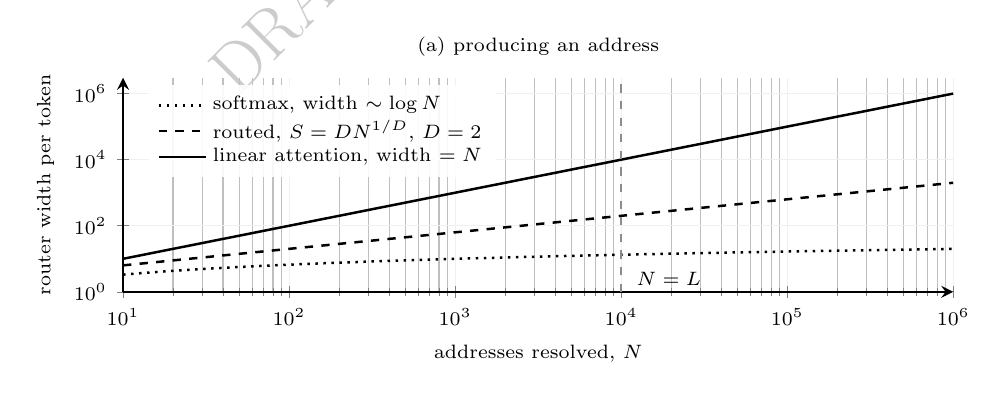
\begin{tikzpicture}
\begin{axis}[
  width=1.0\linewidth, height=4.3cm,
  xmode=log, ymode=log, log basis x=10, log basis y=10,
  domain=10:1e6, samples=60,
  xmin=10, xmax=1e6, ymin=1, ymax=3e6,
  xlabel={addresses resolved, $\Nst$},
  ylabel={router width per token},
  axis lines=left, grid=both, major grid style={gray!12},
  tick label style={font=\scriptsize}, label style={font=\scriptsize},
  legend pos=north west, legend cell align=left,
  legend style={font=\scriptsize, draw=none, fill=white, fill opacity=0.9, text opacity=1, row sep=-2pt},
  title style={font=\scriptsize, yshift=-2pt}, title={(a) producing an address},
  line width=0.9pt,
]
\addplot[black, dotted] {ln(x)/ln(2)};      \addlegendentry{softmax, width $\sim \log \Nst$}
\addplot[black, dashed] {2*sqrt(x)};        \addlegendentry{routed, $\Slv = \Dlv \Nst^{1/\Dlv}$, $\Dlv = 2$}
\addplot[black] {x};                        \addlegendentry{linear attention, width $= \Nst$}
\draw[dashed, black!45] (axis cs:1e4,1) -- (axis cs:1e4,3e6);
\node[font=\scriptsize, anchor=south west, inner sep=1.5pt] at (axis cs:1.15e4,1.1) {$\Nst = L$};
\end{axis}
\end{tikzpicture}
\end{minipage}\hfill
\begin{minipage}[b]{0.49\linewidth}
\centering
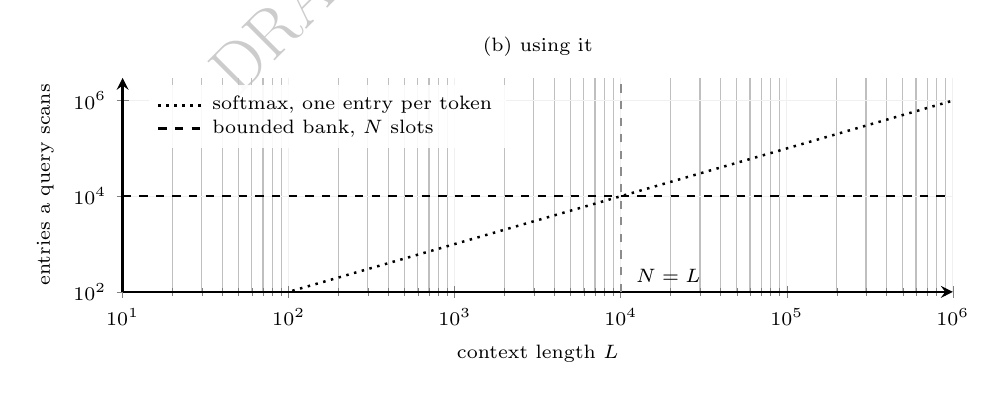
\begin{tikzpicture}
\begin{axis}[
  width=1.0\linewidth, height=4.3cm,
  xmode=log, ymode=log, log basis x=10, log basis y=10,
  domain=10:1e6, samples=60,
  xmin=10, xmax=1e6, ymin=1e2, ymax=3e6,
  xlabel={context length $L$},
  ylabel={entries a query scans},
  axis lines=left, grid=both, major grid style={gray!12},
  tick label style={font=\scriptsize}, label style={font=\scriptsize},
  legend pos=north west, legend cell align=left,
  legend style={font=\scriptsize, draw=none, fill=white, fill opacity=0.9, text opacity=1, row sep=-2pt},
  title style={font=\scriptsize, yshift=-2pt}, title={(b) using it},
  line width=0.9pt,
]
\addplot[black, dotted] {x};                \addlegendentry{softmax, one entry per token}
\addplot[black, dashed] {1e4};              \addlegendentry{bounded bank, $\Nst$ slots}
\draw[dashed, black!45] (axis cs:1e4,1e2) -- (axis cs:1e4,3e6);
\node[font=\scriptsize, anchor=south west, inner sep=1.5pt] at (axis cs:1.15e4,1.2e2) {$\Nst = L$};
\end{axis}
\end{tikzpicture}
\end{minipage}
\caption{\textbf{What an address costs, on both sides.} The abscissa in (a) is the number of slots a design resolves and the ordinate is the router width a token produces to reach them, which is the query--key width for a similarity or a dense feature map and $\Slv = \sum_l \bl$ for a factorized router. Softmax attention's similarity multiplies evidence across dimensions, so $\Theta(\log \Nst)$ features separate $\Nst$ addresses. Linear attention's is a sum over features, so its capacity is the feature dimension itself. A factorized router lies between, at $\Dlv \Nst^{1/\Dlv}$ for fixed depth and logarithmic once depth grows with capacity. Attention is the cheaper producer, and (b) is what it pays for that: its addresses are the tokens themselves, so the entries a query scans grow with the context, where $\Nst$ slots hold whatever the context is. The two meet at $\Nst = L$, where a comparison is capacity-fair (Section~\ref{sec:corner}). The curves are structural laws with constants suppressed.}
\label{fig:space}
\end{figure}

Take a memory whose slots update independently and whose readout is linear, with write and read coefficients that are functions of the input alone. That recurrence is linear attention at feature dimension $\Nst$, its two routing vectors in the roles of key and query features (Section~\ref{sec:reduction}). The statement holds for any router, so it describes the general form of a routed linear-attention head.

RoLA is the head this licenses, and its feature map is factorized. It has $\Dlv$ routing levels, level $l$ offering a choice among $\bl$ branches, with one sparse distribution per level. A leaf is a complete address, one branch chosen at every level, and it names one slot.

Capacity is then the product of the widths where the router's output is their sum, $\prod_l \bl$ slots from $\sum_l \bl$ numbers, which is the mixed-radix arithmetic the design runs on.

The contributions follow that order.
\begin{enumerate}\setlength{\itemsep}{1pt}\setlength{\parskip}{0pt}
\item The reduction, and the recent routed family located in it, including the update rules that fall outside it (Section~\ref{sec:reduction}).
\item The capacity theory that sizes $\Nst$ against what a retrieval contract demands, with the rule that a comparison matches addressing entropy, the log of the number of addresses a design resolves, in place of parameter count (Section~\ref{sec:capacity}). Addressing entropy is, in short, how many distinct places a design can tell apart, counted in bits.
\item The hierarchical entmax feature map, in the three wirings of its read and write supports. Its decay runs on a clock of received write mass, learned per level and held off the gradient, which is what removes the state history from the backward pass (Section~\ref{sec:rola}).
\item The kernel that bills the slots a token touches and not the slots it owns, with the cost model that plans it. It runs at $\Nst = 65{,}536$ and meets attention's arithmetic at $\Nst = L$ (Section~\ref{sec:cost}).
\end{enumerate}

The released layer takes the levels, their widths, each level's activation and side assignment, and the clock as configuration (Appendix~\ref{apd:ladder}).

Language modelling at any scale is the sequel's subject.

% ============================================================
% 2. Bounded-state memories
%
% Budget 0.45 pp (0.75 in the structure, trimmed by the compensating cut
% booked in FILL 3: Sec. 3 as landed already carries the update-rule split in
% its non-reducing-wing paragraph, so the update-rule axis here is one
% paragraph of cost and no taxonomy).
%
% DUPLICATION SWEEP (claims ledger, D1): the update-rule walk was cut to two
% sentences (the axis exists; a sharper write costs parallelism). Sec. 3's P8
% ladder is the survivor and owns the classification, which is what the
% no-taxonomy-here note below always asked for.
%
% Owns nothing, and no displays. None of Sec. 3's taxonomy appears here: the
% split between update rules that reduce and update rules that do not belongs
% to Prop. 1 and is stated there, after the theorem earns it. What this
% section owes is the vocabulary Sec. 3 then uses without defining: linear
% attention's state, the feature dimension as its capacity, the recall gap
% MQAR measures, and the update-rule axis read as a cost ledger.
% ============================================================
\section{Bounded-state memories}
\label{sec:background}

Softmax attention \citep{vaswani2017} and linear attention are two instances of one attention form, an output built by contracting a query against per-token entries whose keys are fixed when written. The kernel reading that groups the two is \citet{tsai2019}'s, and the condition on keys is ours. The name is also used loosely, as an umbrella for the linear-time recurrent family at large, the delta rule and its gated variants included \citep{yang2024fla}. We use it in the strict sense of \citet{katharopoulos2020} throughout, under which the delta rule and its variants fall outside the form, their updates reading as fast weights \citep{schlag2021fwp}. Those authors show the two readings to be formally equivalent, so the boundary is one of scope alone.

Linear attention removes attention's pairwise score. A feature map $\phi$ applied to queries and keys alike writes the similarity as an inner product $\phi(q_t)^\top \phi(k_j)$, so the sum over earlier tokens folds into a running state $M_t = \sum_{j \le t} \phi(k_j) v_j^\top$ \citep{katharopoulos2020}. That state is a matrix of fixed shape, set by the feature dimension $\dqk$ and the width of a value. A read contracts it once against $\phi(q_t)$. Per-token compute and stored state then stop growing with the context.

The feature dimension is also what bounds recall. A stored value survives retrieval only while the feature vector that addressed it stays separable from the rest, so $\dqk$ and not the token count sets how many key-value pairs the state holds at once. Multi-query associative recall makes the gap measurable \citep{arora2023zoology}. A sequence presents many key-value pairs and then queries a subset of the keys. Accuracy falls as the pair count approaches what the feature dimension can separate, where softmax attention holds accuracy by keeping a separate entry per token.

Much of the line since has varied the update rule, and that axis reads as a ledger of what a write may depend on (Appendix~\ref{apd:ladder}).

% ============================================================
% 3. Routed slot memories as linear attention
%
% Owns Prop. 1 (prop:reduction) and two tables: tab:translate, the reduction
% read as a dictionary (it is what licenses the vocabulary phase change: this
% section is the last one written in routing words, and Secs. 4-9 speak linear
% attention); and tab:family, the whole routed family.
%
% TABLE MERGE (user-ratified 2026-08-03): tab:nonreducing is GONE, its rows
% folded into tab:family. Under the three-beat spine both tables held the same
% objects (routed designs = key producers on a recurrence) differing in one
% attribute, so the physical split was the old two-wing boundary surviving as
% furniture. The "Recurrence" column types each row's A_t and SUBSUMES the old
% decay-clock column, decay being the diagonal recurrence's content. The old
% "Where it differs from the form" column is DELETED: it restated the recurrence
% entry as a verdict. The reduction's coverage now reads off the Recurrence
% column, and the caption says so in choice register (Sec. 1's beat-2), not as
% adjudication. Neither table carries a "reduces" column: membership is the
% statement. REGISTER (three-beat reframe,
% 2026-08-03): tab:nonreducing is RELATED WORK, not a contribution-bearing
% exhibit. Its intro states that the beat-1 observation (routing is key
% production) covers those designs unchanged and that what differs is the rule
% the router feeds; it is not an exclusion argument. The column header is
% descriptive ("Where it differs from the form"), and the choice rationale
% lives in Sec. 1's beat-2 paragraph, which this section back-references. The vs.-GDN standings that used to be
% Tab. 1's last column are GONE from the paper entirely: they went with the old
% campaign scope (Sec. 7 header comment, 2026-08-02), and Sec. 7 carries no
% baselines prose about the routed family beyond the no-head-to-head argument.
% Tab. 1's last column is each paper's decay clock instead (sourced per row;
% SSE's row was re-verified against the source on 2026-08-03: its Table 1 says
% "Both SSE and MoM employ diagonal gating, similar to GLA", so the transition
% is diagonal and the clock is a timestep gate, not identity/n.r.; and its
% default read sets T'=T, i.e. dense over all partitions). GDN is a CONTENDER in
% Sec. 7's ladder (vanilla LA, GLA, GDN, softmax attention), not a standing.
%
% MoM CORRECTION (2026-08-01; EQUATION NUMBER RE-VERIFIED 2026-08-03): MoM was
% in tab:family on its framework's general update, M_t = M_{t-1} + k^T v, pure
% additive, the framework being explicitly pluggable across linear-recurrent
% rules. But its experiments "employ the Gated DeltaNet as the memory update
% mechanism", and those experiments are the source of the vs.-GDN standing
% Sec. 7 quotes. The as-published guard therefore puts MoM-as-evaluated in
% tab:nonreducing, where it is now the guard's exhibit rather than its
% counterexample.
%
% The equation number is MoM's Eq. 8, as the tab:nonreducing cell states.
% Source of record: rola-scratch/workflows/paper-pile2-verification/
% mom-sdm-fwpkm.md, which transcribes Sec. 3.2.2's "2. Memory Update: We update
% the activated memory state using k,v: (8)" as M^m_t = M^m_{t-1} + (k^m_t)^T
% v^m_t. Two earlier notes in this header were wrong and are retracted: Eqs. 5-6
% are the router's score/top-k/normalize equations and not a memory update at
% all, and the readout o_t = q_t M_t sits at Eq. 4 in the preliminaries, not at
% Eq. 8.
% Sec. 4 references
% prop:reduction by number; Sec. 5's Prop. 2 is the RoLA instance and is NOT
% stated here.
%
% COMPRESSION RULING (coordinator-directed): the member-by-member walk through
% Tab. 1 is compressed to the table plus one connecting paragraph, with no
% per-row prose, RAM-Net excepted (closest prior work, fullest treatment).
% Quarry for the discarded per-row prose: d95c2c0, 15ec38c, 039db7e.
%
% R5's earlier rejection of this merge (claims ledger, 2026-08-02) is
% SUPERSEDED by the 2026-08-03 ruling above. R5 measured a merge that kept both
% column sets and so paid six n/a cells; it was rejected on that cost, the body
% total being unchanged at 13.651 pp. The ratified merge instead COLLAPSES the
% columns (Recurrence subsumes the decay clock; the verdict column is deleted),
% so no row carries an empty cell, and the ground is the spine rather than page
% height.
%
% tab:phigoal (039db7e) is DISSOLVED, its one home now the connecting paragraph
% after Tab. 1. Merging it into Tab. 1 as a second row block was built and
% measured first: four of the five columns (max slots, reduces, vs. GDN) are
% n/a for a dense fidelity map, so the merge pads the table with empty cells
% and costs 0.11 pp that the compression ruling cannot afford. The contrast is
% one sentence of prose, and it carries the four citations. tab:phigoal no
% longer exists anywhere.
% ============================================================
\section{Routed slot memories as linear attention}
\label{sec:reduction}

This section establishes the identification the rest of the paper runs on: a routed slot memory is linear attention under a particular feature map. Recent bounded-state designs replace linear attention's single recurrent state with a bank of $\Nst$ slots \citep{peng2022abc, zhang2024gsa, afzal2026raven, xiao2026ramnet}. A router decides which slots each token writes and which its query reads.

Read as mechanisms they look like anything but feature maps. The recurrence is indifferent to what produced the vector: a routed slot memory is linear attention under a particular feature map, and the proposition names it.

\begin{proposition}[Routed slot memories are linear attention]
\label{prop:reduction}
Consider a memory of $\Nst$ slots, slot $s$ holding $M_{t,s} \in \R^{\dv}$, driven at token $t$ by a write vector $w_t \in \R^{\Nst}$, a read vector $r_t$, a value $v_t \in \R^{\dv}$ and a retention vector $a_t$, with $M_{t,s} = a_{t,s} M_{t-1,s} + w_{t,s} v_t$ and $y_t = \textstyle\sum_s r_{t,s} M_{t,s}$. Assume slot separability (no cross-slot mixing), input-affine writes ($w_t$, $r_t$, $v_t$ and $a_t$ are functions of the input stream and not of $M$), and a linear readout. Then with $a_{t,s} = 1$ the unrolled recurrence is linear attention at feature dimension $\dqk = \Nst$ under $\phi(k_t) = w_t$, $\phi(q_t) = r_t$, $M_t = \textstyle\sum_{j \le t} \phi(k_j) v_j^\top$; input-dependent $a_{t,s} \in (0,1]$ gives gated linear attention, $a$ acting as a per-feature decay on that map.
\end{proposition}

Separability makes the update $\Nst$ independent scalar recurrences. Affine writes make every coefficient in them a function of the inputs alone, so the sum is a feature map evaluated on the stream (Appendix~\ref{apd:ladder}).

Reading a routed memory that way costs nothing and fixes the vocabulary. Table~\ref{tab:translate} is the dictionary. It is why the sections after this one speak linear attention in place of routing. What a design chooses is a feature map, and the routing words name properties of that map.

\begin{table}[H]
\centering
\scriptsize
\caption{\textbf{The reduction as a dictionary.} Proposition~\ref{prop:reduction} carries the left column onto the right one, each entry an identity rather than an analogy, so what the linear-attention literature already asks of a feature map is what to ask of a router.}
\label{tab:translate}
\setlength{\tabcolsep}{6pt}
\begin{tabular}{@{}ll@{}}
\toprule
Routed slot memory & Linear attention \\
\midrule
write routing $w_t$          & key features $\phi(k_t)$ \\
read routing $r_t$           & query features $\phi(q_t)$ \\
one of the $\Nst$ slots      & one feature dimension \\
the bank, and its contents   & the state $M_t$, at $\dqk = \Nst$ \\
retention $a_{t,s}$          & per-feature gating \\
a level's entmax allocation  & a factor of a sparse feature map, with true zeros \\
a leaf address               & the index of a feature \\
\bottomrule
\end{tabular}
\end{table}

The normalized regime is a fact about RoLA and not a simplification of it, since write mass, the clock reading it and entmax as a projection onto the simplex all need a magnitude only a nonnegative coefficient supplies. Keeping it is what puts the head on softmax attention's ground, and it scopes the paper (Appendix~\ref{apd:ladder}).

The proposition's condition is a condition on the transition, and the field reads as a ladder through it. Every modern fixed-state architecture writes its state $S_t$ as a linear-in-state recurrence $S_t = A_t S_{t-1} + b_t$, with the transition $A_t$ and the input term $b_t$ functions of the input stream alone. What separates the classes is the structure of $A_t$.

The identity is undecayed linear attention. Diagonal transitions are what elementwise decay and gating produce, so an unrolled product of them collapses to a per-token elementwise reweighting the keys absorb. A rank-one modification of the identity fails to commute, and dense $A_t$ is the general linear RNN; Appendix~\ref{apd:ladder} walks the ladder.


Table~\ref{tab:family} collects the family across that ladder, the designs on the diagonal together with the routed ones built on the other recurrence. Their routing is key production like any other, so the reading above covers them all unchanged. What differs is the rule the router feeds, a transition off the diagonal for the delta-rule members and a state-dependent write for the gradient-descent one. The factorization the attention form runs on is unavailable around those.



\begin{table}[H]
\centering
\scriptsize
\caption{\textbf{The routed family as feature maps.} Every row is one recurrence under a produced feature map, its routing key production like any other, so the feature dimension $\Nst$ compares across rows; for the diagonal rows, ours included, Proposition~\ref{prop:reduction} writes that recurrence in the attention form. We read $\Nst$ off the largest configuration each paper reports through that paper's own address formula, $4^5$ from RAM-Net's $d_p^U$ at $d_p = 4$, $U = 5$, $Nc$ from SSE's $N$ partitions over a base row count $c$, and $(d/4H)^2$ from SDM's formula at its 8B width. Where a paper states no factor we leave it symbolic. ``w/r'' is the sparsity of the write and read supports, sp.\ for sparse. The recurrence column types each row's transition $A_t$ with the clock or the rule that fills it, and the diagonal rows are the class this paper works in, the choice Section~\ref{sec:intro} states. In every row but ours the sparsity pattern is a fixed property of the design, where RoLA sets it per level: the default is sparse-write/dense-read, and the level split of Section~\ref{sec:experiments}, one level sparse on the write and another sparse on the read, realizes sparse/sparse. Sparse Delta Memory, abbreviated SDM in the first column, is unrelated to Kanerva's sparse distributed memory \citep{kanerva1988sdm}. FwPKM addresses a product-key bank of $512^2$ slots, and MoM runs four memories and a shared one, classified here as the instantiation it evaluates rather than as its pluggable framework, whose plain-additive form (its Eq.~8) is diagonal.}
\label{tab:family}
\setlength{\tabcolsep}{3pt}
\begin{tabular}{@{}lllll@{}}
\toprule
Method & What $\phi$ is & $\Nst$ & w/r & Recurrence \\
\midrule
Raven \citep{afzal2026raven}   & sigmoid, top-$k$       & 512               & sp./dense   & diagonal, decay on selection \\
RAM-Net \citep{xiao2026ramnet} & Kronecker softmax      & $4^5$             & sp./sp.\    & diagonal, write mass at one global rate \\
SSE \citep{sse2025}            & top-$k$, partitions    & $Nc$              & sp./dense   & diagonal, timestep gate \\
Mamba-2 \citep{dao2024mamba2}  & dense, input-dependent & 256               & dense/dense & diagonal, timestep gate \\
SDM \citep{cabannes2026sdm}    & top-$k$ scores         & $2.3{\times}10^5$ & sp./sp.\    & $I - \beta_t k_t k_t^\top$, the delta rule \\
FwPKM \citep{zhao2026fwpkm}    & product-key top-$k$    & $2.6{\times}10^5$ & sp./sp.\    & state-dependent, a local gradient step \\
MoM \citep{du2025mom}          & softmax, top-$k$       & $5\,\dqk$         & sp./sp.\    & $I - \beta_t k_t k_t^\top$, gated delta as evaluated \\
\addlinespace
RoLA (ours) & mixed-radix entmax & \placeholder{largest trained $\Nst$} & per level & diagonal, per-level write-mass clock, detached \\
\bottomrule
\end{tabular}
\end{table}

Raven, SSE and RoLA write sharply while reading densely, and they pay differently for it (Appendix~\ref{apd:ladder}).

The recurrence off the diagonal gives up the chunked parallel form, which is one of the reasons Section~\ref{sec:intro} gives for taking the affine side. Whether the affine side is itself the limitation is the hypothesis this paper tests (Appendix~\ref{apd:ladder}).

The proposition places every row of the table, ours included, since routing is a way of building a feature map and routing per se is novel nowhere. The form holds for any router, so a routed linear-attention head is a setting of it and not a design beside it. What a proposal still owes is its map, its clock and its kernel.

Three things separate ours from the rest of the family. The first is scale. Our map is exact entmax over a factorization sized for $\Nst$ between $10^5$ and $10^6$, three orders above the $10^2$ to $10^3$ at which the routed alternatives report a trainability fix (Appendix~\ref{apd:ladder}). This paper's kernel addresses $\Nst = 65{,}536$ (Section~\ref{sec:cost}), and Table~\ref{tab:family}'s open cell is the largest trained one.

The second is the decay. Advancing by received write mass is prior art we carve out below; ours are two properties of that clock, a rate learned per level and exact detachment in place of a proxy gradient (Section~\ref{sec:decay}).

The third is a kernel at $\Nst = L$ (Section~\ref{sec:cost}). Without one, describing a slot memory as linear attention at $\dqk = 10^6$ restates the design and does not price it (Appendix~\ref{apd:ladder}).

RAM-Net is the closest prior work and anticipates much of the mechanism, so we state the overlap in full \citep{xiao2026ramnet}. It partitions the input into $U$ sub-vectors, softmaxes each and synthesizes a slot address as their Kronecker product, giving $d_p^U$ slots, then truncates to the top $K$ of them. Its update is affine and key-free, its decay a continuous power of the write weight a slot receives, and it ships sparse kernels that decode addresses without enumerating the product. Factorized product addressing, key-free affine slot writes, a normalized readout over addressed slots and write-driven forgetting belong to that work, and we claim none of them.

What we add is a hierarchy in place of a flat factorization, and exact entmax where RAM-Net truncates a softmax to its top $K$. Our rate is learned per level and detached, where its clock is one global exponent trained through a proxy gradient. Appendix~\ref{apd:ladder} states the overlap and the four differences in full.

% ============================================================
% 4. RoLA
%
% Every equation is verified against
% ROLA_HIERARCHICAL_VALUE_MEMORY_ARCHITECTURE.md rev 2026-07-29.18, which is
% normative for the model mathematics:
%   Eq. (1),(2)  <- arch 4.1 (topology, allocations, level configurations)
%   Eq. (3)      <- arch 4.2 (one mass per side; leaf factors)
%   Eq. (4),(5)  <- arch 4.3 (value recurrence, num/den/readout; the epsilon
%                  convention, here written eta so that epsilon stays free for
%                  the union error carried into Sec. 7)
%   Eq. (6)      <- arch 4.4.2 LeafMassDecay (compact per-branch dials, the
%                  AND-product leaf rate, the detached clock, g_write absent
%                  from the clock, strict complete-leaf immortality)
%   Eq. (7)      <- the touch product, r*w = prod_l b_l = N. SCOPED: it governs
%                  the ALL-COVERAGE wirings only (every level dense on exactly
%                  one side); r and w are STRUCTURAL ENVELOPES, guarantee
%                  widths and not per-token bills, the realized entmax support
%                  sitting at or below them; the shared solve sits at r*w << N
%                  by design. Ratified form recovered from Sec. 7 at ee169ee.
%                  Never write that a token touches r and w, and never state
%                  the product without naming the all-coverage scope.
%   Eq. (8)      <- union split, settled source semantics:
%                  p = entmax((z_r + z_w)/2), sigma = sigmoid(z_r - z_w),
%                  read = p*sigma UNNORMALIZED, write = p*(1-sigma)
%                  RENORMALIZED over supp(p). The AVERAGE (not the sum) is the
%                  settled form (user decision 2026-07-11, recorded in
%                  rola-scratch/workflows/union-split/findings.txt under
%                  "AVERAGE CORRECTION"); rola_bench/named_configs.py still
%                  quotes the superseded sum form in its docstring and is stale
%                  on this point. Re-verified against
%                  rola-standalone/rola/routing/reference.py
%                  (_union_split_with_support).
% WIRING BLOCK (user-ratified restructure, 2026-08-03): the legacy stratification
% is dissolved. sec:wiring "Structural requirements" states the constraint system
% once (single-mechanism premise, the trainability guarantee and the wiring it
% excludes, agreement-or-coverage, the touch pricing of Eq. (7)) and carries NO
% candidate detail. Tab. wirings is the hinge, the derivation's output, placed
% between the requirements and the candidates. Then one small structurally
% parallel subsection per candidate, each in the same internal shape
% (construction, how it buys the guarantee, classification, liability):
% sec:denseread, sec:levelsides, sec:union. The old "The shared-support solve"
% subsection dissolved into sec:union under that shape, and the third-geometry
% paragraph that used to close it became sec:levelsides. One home per sentence:
% Sec. 7 re-contextualizes and states no law sentence of its own.
%
% Capacity claims belong to Sec. 5 and cost claims to Sec. 6; this section
% cross-references both and states neither.
% ============================================================
\section{RoLA}
\label{sec:rola}

This section fixes the head the reduction licenses. A RoLA head keeps a state of $\Nst$ features, and its feature map gives each token key features saying which it writes and query features saying which it reads. Four parts are configurable, and the subsections below fix each: the level configuration, the activation each allocation comes from, the decay semantics, and the readout normalization. Allocations stay normalized and nonnegative, the regime scoped in Section~\ref{sec:reduction}.

\subsection{Topology of the feature map}
\label{sec:topology}

The map is a hierarchy of levels whose complete addresses are its features. Fix one batch element and one head. The map has $\Dlv$ levels, level $l$ of branch width $\bl$. A leaf address picks one branch per level, and the feature count is the product of the widths:
\begin{align}
  s = (d_0, \dots, d_{\Dlv-1}), \qquad d_l \in \{1,\dots,\bl\},
  \qquad \Nst \;=\; \prod_{l=0}^{\Dlv-1} \bl ,
  \label{eq:leafcount}
\end{align}
one feature per leaf. We write $d_l(s)$ for the branch leaf $s$ takes at level $l$, and $\Slv = \sum_l \bl$ for the total branch width. The sum is what a side emits, the product is what it addresses, and the gap is what depth buys. The levels are scales of the address, where log-linear attention makes its hierarchy over the sequence axis \citep{guo2025loglinear}. A coarse level here selects a region of one fixed state, and every token passes through every level.

At token $t$ each side emits one allocation per level, a distribution over that level's branches saying where the side points:
\begin{align}
  p^{\mathrm{r}}_{l,t,d} \ge 0,\quad \textstyle\sum_d p^{\mathrm{r}}_{l,t,d} = 1,
  \qquad
  p^{\mathrm{w}}_{l,t,d} \ge 0,\quad \textstyle\sum_d p^{\mathrm{w}}_{l,t,d} = 1,
  \label{eq:levelalloc}
\end{align}
with $p^{\mathrm{r}}$ the read allocation and $p^{\mathrm{w}}$ the write allocation. Each level and side carries its own activation. Softmax is dense, while the $\alpha$-entmax family returns true zeros \citep{peters2019sparse, martins2016sparsemax}, meaning that a branch left out gets a true zero and not merely a small number. We use its order-$1.5$ member and sparsemax at order $2$.

The support of such a solve is the set of branches it puts mass on, in other words the branches the side actually touches. Everything else gets a true zero. That support has a boundary moving continuously with the logits, so the task gradient recruits and releases branches. We write $\entmaxop$ for whichever order a level carries, and reserve $\alpha$ for the provisioning ratio of Section~\ref{sec:capacity}.

Each level carries one of two configurations, independent or tied, and a tied level is what the shared-support solve of Section~\ref{sec:union} builds on (Appendix~\ref{apd:wirings}).

\begin{figure}[H]
\centering
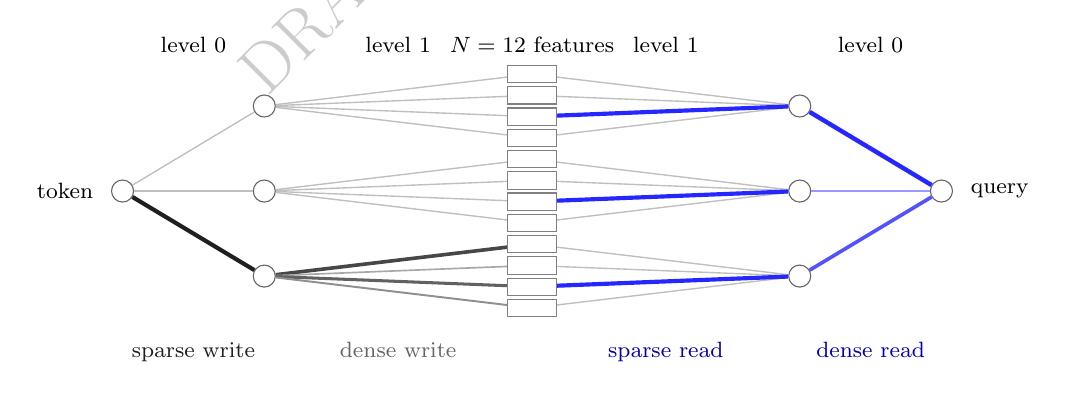
\begin{tikzpicture}[
  lf/.style={draw=black!50, fill=white, minimum width=0.62cm, minimum height=0.22cm, inner sep=0pt},
  nd/.style={draw=black!60, circle, inner sep=1pt, minimum size=0.28cm, fill=white},
  sk/.style={draw=black!25, line width=0.5pt},
  lb/.style={font=\footnotesize},
]
% Horizontal bowtie. The writing token enters at the left and routes through
% its levels into the leaf column; the query enters at the right and routes
% through the same levels into the same column. One distribution per level
% (Eq. 2), so level 1's pattern repeats under every level-0 branch.
% Drawn is the LEVEL SPLIT, the paper's one exported name for this wiring (Sec. 7,
% Tab. 5, App. A). "Split assignment" was an alias for it and is retired
% (settlement fix 2026-08-03: the alias is gone from this caption). The term
% is quarantined out of Sec. 4's prose (style gate B6), which states the geometry
% rather than naming it, so no gloss is owed here; the caption identifies the
% wiring by tab:wirings' own row phrase, "sparsity split by level". Level 0 writes sparsely and reads
% densely, level 1 writes densely and reads sparsely. Bold marks a sparse
% support and graded tint a dense one, black the write side and blue the read.
\foreach \i in {1,...,12}{\coordinate (p\i) at (0,{1.485-0.27*(\i-1)});}
\node[nd] (w1) at (-3.4,1.08) {}; \node[nd] (w2) at (-3.4,0) {}; \node[nd] (w3) at (-3.4,-1.08) {};
\node[nd] (r1) at ( 3.4,1.08) {}; \node[nd] (r2) at ( 3.4,0) {}; \node[nd] (r3) at ( 3.4,-1.08) {};
\node[nd] (tk) at (-5.2,0) {};    \node[nd] (qy) at ( 5.2,0) {};
% write side: sparse at level 0 (one branch, bold), dense at level 1 (tint)
\draw[sk] (tk)--(w1); \draw[sk] (tk)--(w2);
\draw[draw=black!88, line width=1.5pt] (tk)--(w3);
\foreach \j in {1,2,3,4}{\draw[sk] (w1)--(p\j);}
\foreach \j in {5,6,7,8}{\draw[sk] (w2)--(p\j);}
\foreach \j/\w/\o in {9/1.3/72, 10/0.6/34, 11/1.1/62, 12/0.7/44}{
  \draw[draw=black!\o!white, line width=\w pt] (w3)--(p\j);}
% read side: dense at level 0 (tint), sparse at level 1 (one branch each, bold)
\foreach \n/\w/\o in {r1/1.6/85, r2/0.7/40, r3/1.3/68}{
  \draw[draw=blue!\o!white, line width=\w pt] (qy)--(\n);}
\foreach \n/\j in {r1/1, r1/2, r1/4, r2/5, r2/6, r2/8, r3/9, r3/10, r3/12}{
  \draw[sk] (\n)--(p\j);}
\foreach \n/\j in {r1/3, r2/7, r3/11}{
  \draw[draw=blue!85!white, line width=1.5pt] (\n)--(p\j);}
\foreach \i in {1,...,12}{\node[lf] at (p\i) {};}
\node[lb, anchor=east] at (-5.45,0) {token};
\node[lb, anchor=west] at ( 5.45,0) {query};
\node[lb] at (-4.30,1.86) {level $0$};
\node[lb] at (-1.70,1.86) {level $1$};
\node[lb] at ( 0.00,1.86) {$\Nst = 12$ features};
\node[lb] at ( 1.70,1.86) {level $1$};
\node[lb] at ( 4.30,1.86) {level $0$};
\node[lb, anchor=north, black!88] at (-4.30,-1.80) {sparse write};
\node[lb, anchor=north, black!60] at (-1.70,-1.80) {dense write};
\node[lb, anchor=north, blue!70!black] at ( 1.70,-1.80) {sparse read};
\node[lb, anchor=north, blue!70!black] at ( 4.30,-1.80) {dense read};
\end{tikzpicture}
\caption{\textbf{The RoLA head.} Widths $b_0 = 3$ and $b_1 = 4$ give $\Nst = 12$ features, one per leaf address, and that column is the state. The token enters at the left and its query at the right, each passing through the same levels, so level 1's pattern repeats under every level-0 branch. A support drawn bold is sparse and one drawn as graded tint dense, black for the write side and blue for the read, each level assigning the two sides independently. The default configuration is sparse writes and dense reads at every level; drawn here is the sparsity split by level, sparse on the write at level 0 and on the read at level 1, which Section~\ref{sec:experiments} measures.}
\label{fig:head}
\end{figure}

\subsection{Allocation and mass}
\label{sec:allocation}

A write into a leaf carries three jobs, and normalizing the allocation keeps them apart. The allocation says where, one positive scalar per side per token, $g^{\mathrm{r}}_t$ and $g^{\mathrm{w}}_t$, says how much, and the value says what. The gain is the one of the three that reaches the mass alone, which is what makes it identifiable.

Halving the write gain and doubling the value leaves the numerator of the readout below where it was and halves the denominator. The item's weight against everything else the state holds moves, and the output moves with it. Proposition~\ref{prop:identity} carries $g^{\mathrm{w}}_t$ explicitly for that reason. The three jobs give leaf factors
\begin{align}
  R_{t,s} \;=\; g^{\mathrm{r}}_t \prod_{l} p^{\mathrm{r}}_{l,t,d_l(s)},
  \qquad
  W_{t,s} \;=\; g^{\mathrm{w}}_t \prod_{l} p^{\mathrm{w}}_{l,t,d_l(s)} ,
  \label{eq:leaffactors}
\end{align}
with $R_{t,s}$ and $W_{t,s}$ the weights leaf $s$ receives in the read and in the write. Both gains are token-conditioned.

Each side carries one mass and no more, per-level masses collapsing into a side-wide product (Appendix~\ref{apd:wirings}).

\subsection{The value recurrence}
\label{sec:recurrence}

Each leaf owns one value vector $M_{t,s} \in \R^{\dv}$, with $\dv$ the value width. A token deposits its projected value $v_t \in \R^{\dv}$ into every leaf its write factor reaches. Earlier contents survive by a factor $\mathrm{keep}_{t,s} \in (0,1]$ fixed in Section~\ref{sec:decay}, and the read contracts the state:
\begin{align}
  M_{t,s} \;=\; \mathrm{keep}_{t,s}\, M_{t-1,s} \;+\; W_{t,s}\, v_t ,
  \qquad
  \mathrm{num}_t \;=\; \textstyle\sum_{s} R_{t,s}\, M_{t,s} .
  \label{eq:recurrence}
\end{align}
The deposit is additive with input-dependent coefficients, so the recurrence is affine in the state, as Proposition~\ref{prop:reduction} asks.

Each leaf also carries a scalar mass $z_{t,s}$ under the same recurrence, and the readout divides the two contractions:
\begin{align}
  z_{t,s} = \mathrm{keep}_{t,s}\, z_{t-1,s} + W_{t,s},
  \qquad
  \mathrm{den}_t = \textstyle\sum_s R_{t,s}\, z_{t,s},
  \qquad
  y_t = \frac{\mathrm{num}_t}{\mathrm{den}_t + \eta} ,
  \label{eq:global}
\end{align}
with $\eta > 0$ a small constant. The mass is an appended constant-one value channel, and the read gain cancels between numerator and denominator, so we fix $g^{\mathrm{r}}_t = 1$.

The normalized readout has a consequence the rest of the paper leans on. A feature never written contributes zero to $\mathrm{num}_t$ and zero to $\mathrm{den}_t$. Reading it returns nothing rather than noise, so the write support need not contain the read support for correctness, which is what makes the sparse-write, dense-read topology safe.

\subsection{Decay on a write-mass clock}
\label{sec:decay}

With decay disabled, $\mathrm{keep}_{t,s} = 1$ and Eq.~\eqref{eq:recurrence} is additive. The learned form ages a feature by how much it has taken in, not by how long it has existed. In effect, a feature that nothing writes to keeps what it holds indefinitely. Each level carries a per-branch dial $\delta_{l,d} \in [0,1)$, and a leaf's rate is the product of the dials on its own address. The exponent is the write mass that leaf receives at this token, held off the gradient by a stop-gradient $\mathrm{sg}[\cdot]$:
\begin{align}
  w^{\mathrm{leaf}}_{t,s} = \prod_{l} p^{\mathrm{w}}_{l,t,d_l(s)},
  \qquad
  \mathrm{rate}_s = \prod_{l} \delta_{l, d_l(s)},
  \qquad
  \mathrm{keep}_{t,s} = \left( 1 - \mathrm{rate}_s \right)^{\mathrm{sg}[ w^{\mathrm{leaf}}_{t,s} ]} .
  \label{eq:decay}
\end{align}
The write gain $g^{\mathrm{w}}_t$ scales the deposit but stays out of the clock, which keeps the exponent in $[0,1]$.

The clock ignores that gain by design, since a state-dependent share of the accumulated mass would cross the input-affine boundary of Section~\ref{sec:reduction} (Appendix~\ref{apd:clock}).

In the gated linear-attention lineage the clock advances once per timestep, so a feature ages even when it takes no write \citep{yang2024gla, gu2023mamba, yang2024gdn, qin2024hgrn2}. Here an unwritten feature keeps every bit, which is the law we want once Section~\ref{sec:capacity} sizes the state so that almost every feature is idle at almost every step (Appendix~\ref{apd:clock}).

Forgetting in proportion to writing rather than to elapsed time is prior art and we do not claim it, RAM-Net's clock being the closest and Section~\ref{sec:reduction} the carve-out. Raven gates decay on selection \citep{afzal2026raven}, and usage-driven reallocation goes back to the differentiable-memory line \citep{graves2016dnc, rae2016sam}. Two properties of Eq.~\eqref{eq:decay} are ours.

The model learns the rate per level and composes it across the hierarchy. A leaf's rate comes from its own address, at $\Slv$ parameters, so a coarse region can stay durable while the features beneath it turn over.

The clock also runs detached. The stop-gradient leaves the recurrence affine in the state, so the backward pass needs no state history and no chunk-boundary snapshots (Appendix~\ref{apd:proofs}), a claim we scope to the chunked gated-linear-attention family (Appendix~\ref{apd:clock}).

Inside that family we know of no other gate that is an algebraic function of the feature's own write mass, the recent finest-grained forms sharpening the separation of gate from write allocation rather than tying them (Appendix~\ref{apd:clock}).

\subsection{Structural requirements}
\label{sec:wiring}

A head is one mechanism, one bank of leaves under one readout, and a wiring is a choice of how the two sides address it. Gradient reaches the write producer and the value only through the leaves the read gathers. An empty intersection at a step severs that path rather than denting the accuracy. What a wiring owes is therefore a structural intersection and not a probable one, on every step and for every pair of logits. The mechanism under it is entmax's support-restricted Jacobian, which gives an out-of-support logit zero gradient.

Disjoint supports are then permanent dead directions with no re-entry signal, the gap the top-$k$ lineage patches by recruiting with injected noise \citep{shazeer2017moe}; Appendix~\ref{apd:wirings} works the mechanism through.

Correctness survives the cut. Untied sparse supports are exact already, the unwritten leaves of Section~\ref{sec:recurrence} being inert in both sums, and what the intersection buys is gradient rather than exactness (Appendix~\ref{apd:wirings}).

Exactness then classifies what survives that cut, under either of two conditions per level. Under agreement both sides pin the level's digit, at one touch a side, and the cue must carry that digit (Section~\ref{sec:capacity}). Under coverage one side spreads over all $\bl$ digits and asks nothing of the cue there, at $\bl$ touches on that side.

Coverage is what a guarantee for arbitrary logits needs: a read support of size $r_l$ and a write support of size $w_l$ are guaranteed to meet only if $r_l + w_l > \bl$. Concretely, two sets drawn from $\bl$ branches can miss each other unless their sizes together exceed $\bl$.

Touches then price a guarantee, and the arithmetic fixes its width before any measurement. It is the all-coverage wirings the equation below governs, every level supplied dense by one side and none riding on the cue, which is what holds however underdetermined the cue. Such a wiring guarantees a read reaching $r = \prod_l r_l$ leaves and a write reaching $w = \prod_l w_l$, and those two widths multiply to the feature count.
\begin{align}
  r \, w \;=\; \prod_l \bl \;=\; \Nst .
  \label{eq:touchproduct}
\end{align}
That is Eq.~\eqref{eq:leafcount} read on the supports in place of the widths, so structural coupling with each side solving its own support is conserved work along a hyperbola. It scopes to those wirings and is not a requirement of exact addressing.

A contract whose cue determines the address at every level runs at $r = w = 1$ and still reaches all $\Nst$ features, and $r w < \Nst$ says some levels ride on agreement in place of coverage, which is where the shared solve sits by design. The two counts are structural envelopes and not per-token bills: entmax support is adaptive, a token's realized support sits at or below the envelope, and a confident cue collapses toward the point case. The kernel bills the touches a token realizes (Section~\ref{sec:cost}).

A guarantee holding for every pair of logits means at least one side's realized support departs from an independent point mass. Table~\ref{tab:wirings} is what that leaves, and the subsections below construct the three wirings that pay; Appendix~\ref{apd:wirings} derives the family as the guarantee's solution set.

\begin{table}[H]
\centering
\scriptsize
\caption{\textbf{The wiring family.} Each row buys the intersection of Section~\ref{sec:wiring} differently, and the subsections below construct the three that buy it at all. The envelope is the guarantee's width rather than a token's bill, and Eq.~\eqref{eq:touchproduct} governs the first two rows, which supply every level dense on one side. The shared support sits below the hyperbola by design, at both sides sparse. The last row is the wiring the law excludes, cheapest on both sides and structurally unable to promise an intersection at any step.}
\label{tab:wirings}
\setlength{\tabcolsep}{4pt}
\begin{tabular}{@{}l l >{\raggedright\arraybackslash}p{0.21\textwidth} l l >{\raggedright\arraybackslash}p{0.20\textwidth}@{}}
\toprule
Wiring & Pays with & Sides per level & Envelope $(r,w)$ & Touches & Exposure \\
\midrule
Sparse write, dense read & touches   & write pins, read dense, at every level         & $(\Nst, 1)$                        & $O(\Nst)$        & none on either side \\
Sparsity split by level  & structure & each level dense on one side, sparse on the other & $(\sqrt{\Nst}, \sqrt{\Nst})$       & $O(\sqrt{\Nst})$ & a block write, leaking mass into neighbors \\
Shared support           & coupling  & one support serving both sides                 & $r w \ll \Nst$                     & $O(1)$           & a cue diverging from the content, priced by $\varepsilon$ \\
\addlinespace
Untied sparse (excluded) & nothing   & both sides sparse, independently solved        & $(1,1)$                            & $O(1)$           & no guaranteed intersection \\
\bottomrule
\end{tabular}
\end{table}

\subsection{Dense reads}
\label{sec:denseread}

A dense read spreads over every branch of every level while the write stays a point mass, so the read support is the whole state and the write is one leaf. It is the configuration Section~\ref{sec:topology} names the default, and the one Eq.~\eqref{eq:parity} prices at $\Nst = L$ (Appendix~\ref{apd:wirings}).

What it pays is touches, at the envelope $(\Nst, 1)$ of Table~\ref{tab:wirings}: the only sparsity a kernel can harvest is on the write side (Appendix~\ref{apd:wirings}).

\subsection{Sparsity split by level}
\label{sec:levelsides}

Because a leaf factor is a product over levels, the two sides can take their sparsity at different levels, which is the split Table~\ref{tab:wirings} places at $(\sqrt{\Nst}, \sqrt{\Nst})$ (Appendix~\ref{apd:wirings}).

The payment lands on the write, which becomes a contiguous block of features and leaks mass into its neighbours (Appendix~\ref{apd:wirings}).

\subsection{The shared-support solve}
\label{sec:union}

A shared-support level solves once on the averaged logits and splits the two sides inside the resulting support, which makes the intersection an identity and sparsifies both sides at once:
\begin{align}
  p \;=\; \entmaxop\!\left( \tfrac{1}{2}\left(z^{\mathrm{r}} + z^{\mathrm{w}}\right) \right),
  \qquad
  \sigma \;=\; \mathrm{sigmoid}\!\left( z^{\mathrm{r}} - z^{\mathrm{w}} \right),
  \label{eq:union}
\end{align}
with $z^{\mathrm{r}}$ and $z^{\mathrm{w}}$ the level's read and write logits. The read allocation is $p \sigma$ without renormalization, and the write allocation is $p (1-\sigma)$ renormalized over the support of $p$.

A uniform scale on the read side cancels in the ratio of Eq.~\eqref{eq:global}, so leaving the read unnormalized costs nothing. The write allocation must be a distribution, because it deposits mass.%
% PROVENANCE: settled 2026-07-10 (rola-scratch/workflows/union-split/findings.txt).
% Support logits CORRECTED from the sum to the average by user decision
% 2026-07-11, recorded in that file under "AVERAGE CORRECTION" and mirrored
% across the reference and CUDA producers. rola_bench/named_configs.py still
% quotes the sum form in its docstring; that docstring is stale.
{} The two sides stay untied in value through $\sigma$ while sharing one support. Averaging, in place of summing, keeps the tied case an identity, since $\entmaxop(2z)$ and $\entmaxop(z)$ differ.

This is the deliberate exception at the agreement end, both sides sparse at $O(1)$ touches and $r w \ll \Nst$, its exactness resting on the one map sending a cue where the content went rather than on coverage (Appendix~\ref{apd:wirings}).



We write $\varepsilon$ for the resulting task-level error, what a shared support costs: it measures how often a task reads outside where it writes, or the reverse, strongly enough for one support to get it wrong. Its two sources are decomposed in Appendix~\ref{apd:proofs} and its exposure in Appendix~\ref{apd:wirings}.


% ============================================================
% 5. Capacity and addressing
%
% Every theorem-grade statement is verified against
% ROLA_HIERARCHICAL_VALUE_MEMORY_ARCHITECTURE.md rev 2026-07-29.18, which is
% normative for the capacity theory. Line references are to that file:
%   Prop. 2 + rider        <- 5.1 (lines 805-828): Kronecker identity at
%                             d_qk = N = prod b_l; product-vs-sum gap;
%                             "full-rank memory, factorized addressing"
%   provisioning/commit    <- 5.2 (lines 830-843)
%   addressing entropy     <- 5.2 (lines 845-857)
%   bench rule             <- 5.2 (lines 859-864), normative for the paper
%   T0 injectivity         <- 7  (lines 1323-1329)
%   not self-verifying     <- 7  (lines 1331-1345), including the CORRECTION of
%                             the co-occurrence theorems' scope: "items that
%                             never co-occur may share a state" is a STORAGE
%                             claim and survives only where the query's feature
%                             covers everything that can land in the slot.
%                             SELF-VERIFICATION CORRECTED (user ruling
%                             2026-08-03, pending merge into the architecture
%                             doc): the source's asymmetry, attention scoring
%                             the stored key so a wrong match reads low while a
%                             grid read substitutes with no signal, is FALSE as
%                             stated. Both readouts are normalized
%                             kernel-weighted averages, so neither carries an
%                             intrinsic alarm: a query matching nothing still
%                             returns a confident blend, and in the overloaded
%                             regime (demand beyond the distinguishable
%                             directions a width provisions) stored addresses
%                             interfere and weight lands on wrong content at
%                             full confidence. Both are bound by the one law,
%                             demand against allocated addressing capacity, and
%                             both fail confidently-wrong. The surviving
%                             asymmetry is graded (key kept as data, per
%                             occurrence) versus quantized (identity folded
%                             into the address at write, residual discarded)
%                             failure, plus how much capacity a unit of width
%                             buys: a regime difference, not a verification
%                             difference. The sharing-safety condition above is
%                             unaffected and stands. Siblings corrected in the
%                             same pass: Sec. 8's structural-limits sentence
%                             and App. A's post-Lem. 2 rider.
%   T1 disjoint family     <- 7  (lines 1383-1395)
%   T2 general rule        <- 7  (lines 1396-1400)
%   T3 agreement law       <- 7  (lines 1401-1406)
%   contract trichotomy    <- 7  (lines 1407-1416). The old Tab. 2 was collapsed
%                             into prose in the coloring rewrite; its rows are
%                             the family STRUCTURES and the known-in-advance vs
%                             measured split, both preserved there. The shared
%                             case is the realized graph's chromatic number and
%                             NOT |V|: the source marks it "no -- measured" and
%                             |V| is only sufficient.
%   alpha                  <- 7  (lines 1310-1321). The source's other two ratios
%                             are gone: slack (budget - usage) was CUT in the
%                             claims-ledger orphan sweep (ORPHAN 6), and the
%                             margin beta (with K_eff) was CUT in the coloring
%                             rewrite, its load-bearing content surviving as the
%                             existence-vs-learnability sentence in prose.
%   alpha < 1 as aliasing  <- 7  (lines 1367-1376)
%   depth-dynamism         <- 7  (lines 1427-1435)
%   two residual gaps      <- 5.2 (lines 866-878)
%   normalization is not   <- 5.2 (lines 880-895). DUPLICATION SWEEP (D2): the
%                             paragraph is one back-reference sentence now;
%                             Sec. 3's P6 is the survivor, since that is where
%                             the regime scopes Prop. 1.
%
% COLORING PROVENANCE. The graph-coloring formulation of 5.2 (the union
% co-occurrence graph over items; required N = its chromatic number; the
% adversarial, disjoint and interval regimes; the three reductions that license
% sizing below the adversarial demand) goes BEYOND rev .18 of the architecture
% document. Its source of record is
% development/plans/V3_CAPACITY_THEORY_NOTES_2026-07-29.md, section
% "2026-08-03: Coloring formulation (ratified)", pending merge into the
% architecture doc. The graph facts it uses (a complete graph on k nodes needs k
% colors; a multipartite graph is colored by its parts; interval graphs are
% perfect) are textbook, so the rewrite adds no new theorem-grade risk. The same
% section records the retirement of the clique vocabulary, of beta/K_eff, and of
% the contract table, and (2026-08-03 rider) the GRAPH-FIRST ruling this pass
% enforces: no quantity is stated as a bound in its own right, every demand is
% the chromatic number of a named graph, and L, |V| and window widths appear
% only as parameters of the construction that produced that graph. The
% organizing statement sits in 5.2 after the graph paragraph. Fig. 1(b)'s edge
% set is a union of transversal triangles, since a full-length sequence realizes
% one item per position and asks for all of them, so no realized node is
% isolated or joined only inside its column.
%
% COMPRESSION RULING (fill-time; recorded in the findings doc). The quarry
% deposit's four-case 2x2 is NOT built as a display. Its two exactness facts are
% one sentence each inside the failure law, and one of them (unwritten slots are
% inert) is already stated in Sec. 4 after Eq. (5), so restating it here would
% break one-home. The four cases carry no content beyond "they differ in
% exposure surface", which is one clause. A display would spend ~0.15 pp
% restating a one-line law.
%
% GLOSSARY AMENDMENT (user ruling 2026-08-03, pending merge into CLAUDE.md and
% STYLE_DISTILLATION.md): "discrimination" is RATIFIED vocabulary and stays in
% this section's prose (5.2's two-resources paragraph and the sharing-safety
% paragraph). CLAUDE.md line 266 retires it in favour of "addressing capacity",
% which STYLE_DISTILLATION.md 4.1 cuts outright, so the two rulebooks could not
% both be satisfied here. The ruling keeps the word and amends the rulebooks;
% tools/style_whitelist.json carries it on the survivor list with the same note.
% This is a vocabulary ratification, not a gate waiver.
%
% NOTATION: alpha is the provisioning ratio N/L here, per the ratified capacity
% vocabulary. Sec. 4 was edited in the same commit so that alpha is no longer a
% free symbol there (the sparse activation family keeps its standard name
% "alpha-entmax" and its orders are given as numbers).
% ============================================================
\section{Capacity and addressing}
\label{sec:capacity}

Under Proposition~\ref{prop:reduction} RoLA's capacity is a feature dimension, and its addressing is the structure of its feature map. The proposition names it: level widths multiply into capacity, while the map emits only their sum (Section~\ref{sec:topology}).

\begin{proposition}[Kronecker-structured linear attention]
\label{prop:identity}
Unrolled with decay disabled, a RoLA head is linear attention at feature dimension $\dqk = \Nst$ under $\phi(k_t) = g^{\mathrm{w}}_t \bigotimes_l p^{\mathrm{w}}_{l,t}$ and $\phi(q_t) = \bigotimes_l p^{\mathrm{r}}_{l,t}$, each a tensor product of $\Dlv$ normalized allocations of widths $\bl$. The write gain of Eq.~\eqref{eq:leaffactors} scales the deposit, and the read gain is fixed at $g^{\mathrm{r}}_t = 1$ by the normalized readout of Eq.~\eqref{eq:global}. Capacity is their product $\Nst = \prod_l \bl$ and the map emits their sum $\Slv = \sum_l \bl$ per side.
\end{proposition}

That gap is what depth buys, and the map pays for it. The feature vector is a product of per-level marginals, so some patterns over leaves are unreachable while the state itself stays full rank (Appendix~\ref{apd:capacity}).

Factorization costs nothing where writes want point masses, since a delta on a leaf is the product of the per-level digit deltas; it charges spread read patterns instead (Appendix~\ref{apd:capacity}).

Attention provisions $\exp(\Theta(\dqk))$ near-orthogonal directions and materializes $O(L)$ of them per sequence as its cache, where RoLA provisions $\Nst$ combinatorially and commits the features written into. Both are logarithmic-class addressing for an exponential space, and Appendix~\ref{apd:capacity} places that reading against the Hopfield capacity line and the worst-case recall bounds.


The quantity that compares them is addressing entropy: $\log \Nst = \sum_l \log \bl$ for the state, $c\,\dqk$ for a feature map of dimension $\dqk$, with $c$ a packing constant set by the interference one tolerates. Section~\ref{sec:theorygrid} measures $c$ by fitting it. Comparisons match on that quantity, not on parameter count: equalizing parameters while leaving one side an exponentially larger address space measures the mismatch, not the architecture.

\subsection{Vocabulary families and retrieval contracts}
\label{sec:families}

What a head must address is which distinguishable symbols can occur at each position, the family $V_1,\dots,V_L$, and every statement below quantifies over such a family. Token identity gives the shared family and positional encoding the disjoint one, so those are the content-associative and positional cases (Appendix~\ref{apd:regimes}).

A retrieval contract is, in short, the list of questions a task will ask the memory. Each query names a target weighting over the values its sequence wrote, and nothing in it says where those values sit. The pair of maps is a solver, and placement is design freedom.

Under the normalized readout of Eq.~\eqref{eq:global} that solver has two error-free cases, a read confined to features holding one value each and a read spreading over features the sequence never wrote (Appendix~\ref{apd:capacity}).


\subsection{Sizing}
\label{sec:sizing}

Sizing starts from injectivity, which means that no two histories may end up as the same memory. The state loses nothing to the pigeonhole if and only if the map from sequence to written configuration is one-to-one. An injective addressing is available whenever the items a family can present at one position number at most $\Nst$ (Appendix~\ref{apd:regimes}).

We size for point-write assignment, each item entering one feature. An assignment that spreads an item over several features answers to the nonnegative rank of the contract matrix in place of a coloring. Against the contracts this paper instruments that bound degenerates to the one point writes already give (Appendix~\ref{apd:nonneg}).

Above the injectivity floor the binding object is a graph. Its nodes are the items a family can present, one node per item and not one per occurrence, and an edge joins two items when some sequence the distribution realizes asks for both of them separately. An assignment is a coloring of that graph, proper, no edge with one color at both ends, when the write map is injective on every set of items live at once.

Every feature then holds at most one live value, which is the first exact case above. The least $\Nst$ that serves the contract is the chromatic number of that graph (Figure~\ref{fig:coloring}). That is, the head needs one feature for every item a read has to keep apart at the same time.

Every quantity this paper calls a demand is that number evaluated on a particular graph, and provisioning to it leaves every fulfillment pattern available (Appendix~\ref{apd:regimes}).

The quantity is also computable with certificates on the families the instrument builds, so Section~\ref{sec:theorygrid} stamps a solved demand on a cell before it trains.

% R3 (cut plan, 2026-08-03): the three regimes were a 170w enumeration on the
% p8-p9 wall. Absorbed into tab:regimes at regime / graph / chromatic number /
% what it asks of N, which is the four facts each sentence carried. The two
% riders that are NOT per-regime facts (the guarantee tier the grid
% instruments, and the factorization expressing the positional coloring at S
% parameters) keep their sentences below the table, being claims about this
% paper rather than about the graphs.
Three regimes settle that number, and Table~\ref{tab:regimes} is the three.

\begin{table}[H]
\centering
\scriptsize
\setlength{\tabcolsep}{3pt}
\caption{\textbf{Three regimes and the chromatic number each carries.} The graph is the one the distribution realizes, and the least $\Nst$ that serves the contract is its chromatic number.}
\label{tab:regimes}
\begin{tabular}{@{}>{\raggedright\arraybackslash}p{3.3cm}>{\raggedright\arraybackslash}p{4.6cm}>{\raggedright\arraybackslash}p{2.9cm}>{\raggedright\arraybackslash}p{3.9cm}@{}}
\toprule
Regime & Graph it realizes & Chromatic number & What it asks of $\Nst$ \\
\midrule
Random draws over a shared vocabulary & complete on $\min(L, |V|)$ items & $\min(L, |V|)$, a complete graph on $k$ nodes taking $k$ colors & $\Nst \gtrsim \min(L, |V|)$ for exact recall \\
A disjoint family, one vocabulary a position & $L$-partite, so coloring by position is proper however dense the edges between positions grow & $L$ & $\Nst \gtrsim L$: vocabulary size multiplies the nodes and never the colors \\
A recency contract, reads never demanding a superseded item apart & interval overlap, and interval graphs are perfect & the window width, the most items live at one time & $\Nst \gtrsim$ that width, below the count a sequence writes \\
\bottomrule
\end{tabular}
\end{table}

Table~\ref{tab:regimes}'s three regimes are walked through in Appendix~\ref{apd:regimes}: the first is what random draws over a shared vocabulary present, and the instrument of Section~\ref{sec:theorygrid} runs in it, for that guarantee tier.

The third is induced by the contract, and its width is fixed before any architecture is chosen.

\begin{figure}[H]
\centering
\begin{minipage}[b]{0.47\linewidth}
\centering
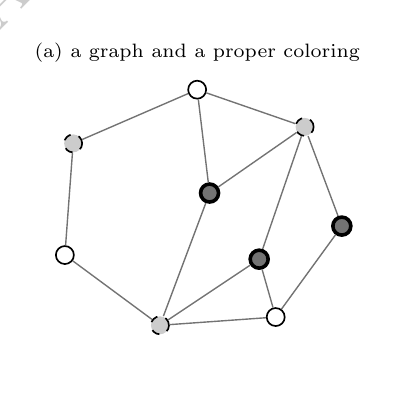
\begin{tikzpicture}[x=1.05cm, y=1.05cm,
  cA/.style={circle, draw=black, line width=0.6pt, fill=white, inner sep=0pt, minimum size=6.5pt},
  cB/.style={circle, draw=black, dashed, line width=0.6pt, fill=black!20, inner sep=0pt, minimum size=6.5pt},
  cC/.style={circle, draw=black, line width=1.3pt, fill=black!55, inner sep=0pt, minimum size=6.5pt},
  ed/.style={draw=black!55, line width=0.5pt}]
\useasboundingbox (-2.05,-1.95) rectangle (2.05,2.25);
\node[font=\scriptsize] at (0,1.95) {(a) a graph and a proper coloring};
\node[cA] (n1) at (0,1.5) {};
\node[cB] (n2) at (1.3,1.05) {};
\node[cC] (n3) at (1.75,-0.15) {};
\node[cA] (n4) at (0.95,-1.25) {};
\node[cB] (n5) at (-0.45,-1.35) {};
\node[cA] (n6) at (-1.6,-0.5) {};
\node[cB] (n7) at (-1.5,0.85) {};
\node[cC] (n8) at (0.15,0.25) {};
\node[cC] (n9) at (0.75,-0.55) {};
\draw[ed] (n1)--(n2); \draw[ed] (n2)--(n3); \draw[ed] (n3)--(n4);
\draw[ed] (n4)--(n5); \draw[ed] (n5)--(n6); \draw[ed] (n6)--(n7);
\draw[ed] (n7)--(n1); \draw[ed] (n1)--(n8); \draw[ed] (n2)--(n8);
\draw[ed] (n5)--(n8); \draw[ed] (n4)--(n9); \draw[ed] (n5)--(n9);
\draw[ed] (n2)--(n9);
\end{tikzpicture}
\end{minipage}\hfill
\begin{minipage}[b]{0.47\linewidth}
\centering
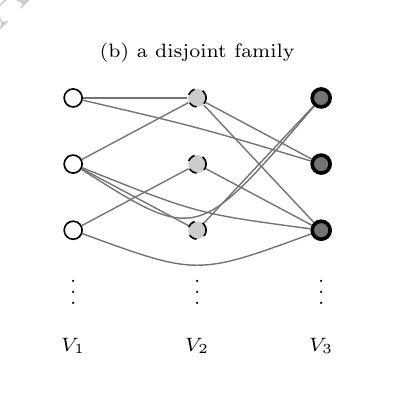
\begin{tikzpicture}[x=1.05cm, y=1.05cm,
  cA/.style={circle, draw=black, line width=0.6pt, fill=white, inner sep=0pt, minimum size=6.5pt},
  cB/.style={circle, draw=black, dashed, line width=0.6pt, fill=black!20, inner sep=0pt, minimum size=6.5pt},
  cC/.style={circle, draw=black, line width=1.3pt, fill=black!55, inner sep=0pt, minimum size=6.5pt},
  ed/.style={draw=black!55, line width=0.5pt}]
\useasboundingbox (-2.05,-1.95) rectangle (2.05,2.25);
\node[font=\scriptsize] at (0,1.95) {(b) a disjoint family};
\node[cA] (a1) at (-1.5,1.4) {}; \node[cA] (a2) at (-1.5,0.6) {}; \node[cA] (a3) at (-1.5,-0.2) {};
\node[cB] (b1) at (0,1.4) {};    \node[cB] (b2) at (0,0.6) {};    \node[cB] (b3) at (0,-0.2) {};
\node[cC] (c1) at (1.5,1.4) {};  \node[cC] (c2) at (1.5,0.6) {};  \node[cC] (c3) at (1.5,-0.2) {};
% Each drawn sequence realizes one item per position and asks for all of them,
% so the edge set is a union of transversal triangles: (a1,b1,c2), (a2,b3,c1),
% (a3,b2,c3), (a2,b1,c3). Every node lies in one, and no node is isolated or
% joined only inside its column. The A--C sides are bowed through the gaps
% between the middle column's nodes.
\draw[ed] (a1)--(b1); \draw[ed] (a2)--(b3); \draw[ed] (a3)--(b2);
\draw[ed] (a2)--(b1);
\draw[ed] (b1)--(c2); \draw[ed] (b3)--(c1); \draw[ed] (b2)--(c3);
\draw[ed] (b1)--(c3);
\draw[ed] (a1) .. controls (0,1.05) .. (c2);
\draw[ed] (a2) .. controls (0,-0.35) .. (c1);
\draw[ed] (a3) .. controls (0,-0.75) .. (c3);
\draw[ed] (a2) .. controls (0,0.0) .. (c3);
\node[font=\scriptsize] at (-1.5,-0.85) {$\vdots$};
\node[font=\scriptsize] at (0,-0.85) {$\vdots$};
\node[font=\scriptsize] at (1.5,-0.85) {$\vdots$};
\node[font=\scriptsize] at (-1.5,-1.6) {$V_1$};
\node[font=\scriptsize] at (0,-1.6) {$V_2$};
\node[font=\scriptsize] at (1.5,-1.6) {$V_3$};
\end{tikzpicture}
\end{minipage}
\caption{\textbf{Sizing as a coloring.} Nodes in (a) are the items a family can present, an edge joins two items some sequence asks for separately, and an assignment of items to features is a coloring, proper when no edge takes one color at both ends. The number of features the contract requires is the chromatic number, three here, and the triangle is what rules two out. Panel (b) is the disjoint family, one column per position: no edge lies inside a column, since symbols at one position never co-occur, so the columns grow as tall as the vocabularies $V_i$ are large while coloring by position stays proper however dense the edges between columns become. A sequence realizes one item per position and asks for all of them, so it contributes a triangle across the columns and every item a sequence realizes carries edges into every other position; the drawn edges are four such sequences. The chromatic number is the column count, and that coloring is the one a factorized map expresses at $\Slv$ parameters, levels as position digits.}
\label{fig:coloring}
\end{figure}

A contract bills two resources, and features are only the first: coloring the graph is a storage statement, and the width a cue must carry to select among the colors is the second (Appendix~\ref{apd:regimes}).


Whether the maps can serve a contract is a relation between two functions on the family. Write $\mathrm{addr}^{\mathrm{w}}$ and $\mathrm{addr}^{\mathrm{r}}$ for the addresses the two sides assign. A contract sending a query symbol $u$ to the stored symbol $\pi(u)$ is served when they agree:
\begin{align}
  \mathrm{addr}^{\mathrm{r}}(u) \;=\; \mathrm{addr}^{\mathrm{w}}\!\left(\pi(u)\right)
  \quad \text{for every } u ,
  \label{eq:agree}
\end{align}
Otherwise the read marginalizes densely over the digits it cannot fix, at an active-leaf count proportional to the matching instances, the bill attention pays for a multi-match query (Lemma~\ref{lem:agree}). Attention satisfies Eq.~\eqref{eq:agree} implicitly, $q \cdot k$ discriminating when the query carries what the key encoded.

The provisioning ratio $\alpha = \Nst / L$ is the dial a design sets. It says, roughly, how many features the head carries per token of context. What it buys is room for a coloring, and a coloring that exists settles neither that the map can express it nor that training finds one. The map realizes only the colorings that factor into a linear entmax classification per level. That is the hypothesis the grid of Section~\ref{sec:theorygrid} tests.

The number a contract requires is thus a functional of the distribution and the contract rather than a property of the head. What changes across families is how one comes to know it: a disjoint family asks for $L$ and a designer knows that in advance, where a shared family asks for a chromatic number only measurement returns. This paper measures neither (Appendix~\ref{apd:regimes}).

Sharing one feature between two symbols is safe when no retrieval map in the contract addresses one of them without the other. Two symbols that never co-occur may then share a feature for storage but not for retrieval, unless the cue the query addresses with covers everything that can land there (Appendix~\ref{apd:sharing}).

None of this asks the map to be computed per sequence, layer 1's family being the token vocabulary and depth supplying the dynamism thereafter (Appendix~\ref{apd:regimes}).

How $\Nst$ must scale with $L$ is a property of the sequences a task realizes rather than of $L$ alone, and the general sizing question is one this paper leaves open (Appendix~\ref{apd:regimes}).


Provisioning below the adversarial demand is a bet that the graph a design faces is smaller than the adversarial one, and Appendix~\ref{apd:regimes} gives the three things that shrink it.



\subsection{$\Nst = L$ as the adversarial contract}
\label{sec:corner}

At $\Nst = L$ the write side can be injective on instances, one color per occurrence, which covers the adversarial completion's demand whatever graph a sequence realizes. Every feature then holds one value, the failure mode above is structurally unavailable, and residual error lies on the read side alone. Softmax attention hardcodes this regime: its addresses are free, one per occurrence and injective by position, so its key map learns what a key encodes and never where it lands.


That regime is an entry fee. Real sequences are redundant, so provisioning $\Nst = \alpha L$ sizes the state to the information in a context rather than to its token count (Appendix~\ref{apd:regimes}).

Setting $\alpha < 1$ is thus a choice of what may alias: provisioning below the chromatic number forces edges to take one color at both ends (Figure~\ref{fig:coloring}). Entmax triage is what chooses the cheap ones, with leaf mass decay metering the turnover of the features that stay hot (Section~\ref{sec:decay}). Parity at $\Nst = L$ is the worst-case guarantee, and $\alpha$ is set from the costly-edge subgraph a distribution presents, which this paper leaves unmeasured.


% ============================================================
% 6. Cost
%
% GOAL (PAPER_STRUCTURE.md): sparse-memory work is billed per tile touched,
% support clustering rather than support size is the cost variable, and RoLA
% meets attention's FLOP count at N = L.
%
% PROVENANCE RULING (2026-08-02, user). The paper prints only ANALYTIC
% quantities (derived FLOP counts, structural counts, asymptotics) and
% measurements with PUBLISHABLE provenance (rental-class hardware, ratified
% protocol). Every constant below was taken on one consumer card with
% single-launch counters, so NONE of it may be printed: the quanta table's work
% column, the quanta statistics (0.97 / 0.606 / 39 %), the gather A/B
% percentages, the timing ratio, the selection counts and the residuals are all
% DEMOTED to \placeholder / \TODO in the rendered text. The block below is the
% provenance record for the re-measurement, not a source to re-inline from.
%
% NUMBERS. Every constant is READ BACK from the committed cost model,
% `rola/planner/schedule.py` in the standalone package (the file the planner
% selects with), not from the earlier draft and not from memory:
%   GATHER_CANDIDATE_FIXED_WORK   = 177.75    per candidate (owner, tile) pair
%   GATHER_CANDIDATE_QUANTUM_WORK = 525.125   per ceil(BC/16) quantum
%   READOUT_FOLD_KSTEP_WORK       = 1755.0    per k-step
%   INTRA_GRAM_KSTEP_WORK         = 144.0     per k-step
%   DECAY_KSTEP_WORK              = (1106.3 + 959.7) / 2 = 1033.0 per k-step
% The gather is NOT the single ~2278 of the earlier draft: 2278.25 is what the
% BC = 64 cell measures per tile, and the two-point solve over ceil(BC/16)
% against the BC = 16 cell (702.88) splits it into 525.125 per quantum plus a
% 177.75 per-tile intercept. Pricing it as one constant made compaction
% unreachable at BC = 16. Provenance for the solve: rewrite.md Secs. 2.20, 2.33,
% and the constant's own docstring block in schedule.py.
%
% Instrument, all constants: RTX 3080 Ti, `ncu --clock-control base`,
% `smsp__inst_executed.sum`, ONE profiled launch per arm, flock-serialized;
% cells from the frozen registry in `benchmarks/bench_consumer_new.py`.
% Isolating cells: GATHER_* from topo-D2-w64x64-BC64 against topo-D2-w64x16-BC16
% (unions saturate at both, so gathering changes no extent and only the dense
% quantum differs); READOUT_FOLD from atscale-L2048, where extents do move;
% INTRA_GRAM from wk1-D2-w64x64-BC64 against topo-D2-w64x64-BC64, which differ
% only in the intra extent KI; DECAY from the BC = 64 / BC = 16 pair at both
% compact arms, which differ only in the k-step count.
%
% atscale-L2048 config, read back from bench_consumer_new.py: widths (256, 256),
% so N = 65536 at D = 2; B = 1, H = 8, d_v = 64, T = 2048, BC = 64, BT = 16;
% order-1.5 entmax routing PRODUCED by a real RoLA layer (route_W scaled 8.0,
% seed 0) with the plan chosen by the planner. Quanta stats (--mode gatherstats,
% rewrite.md Sec. 2.20): mean K / BC = 0.97, readout k-steps 0.606 of 4, ~39 % of
% candidate pairs gather K = 0. Compaction A/B at that cell: 1812.1 M -> 1035.0 M
% instructions (-42.9 %) at decay = None and 2719.6 M -> 1092.6 M (-59.8 %) with
% decay; paired interleaved timing 8.457 -> 6.383 ms (x0.753, IQR 0.094).
% Dense toll, topo-D2-w64x64-BC64: 9.410 M -> 11.743 M (+24.8 %) and
% 13.888 M -> 15.786 M (+13.7 %).
%
% RESIDUALS (rewrite.md Secs. 2.36-2.37, and the landed test
% `test_the_absolute_instruction_totals_are_a_RECORDING_not_an_assertion`):
% the model reproduces 8 of 8 measured joint (BT, compact) argmins, which is what
% binds the constants; its ABSOLUTE totals are recorded, not asserted, at up to
% +83.9 % with the un-identified per-tile term and -61.0 % (one-sided) without
% it. Decay is overpriced by 2.3x on the one at-scale compact cell (453 measured
% against 1033), stated as a direction rather than fitted with a second constant.
% The earlier draft's "reproduces on a minority of cells, one residual of 2.3x"
% is STALE: that was the pre-calibration state.
%
% The 1.5-2x cost of making both sides dense is NOT quoted as a number: no
% in-tree measurement was found for it, so the rider is stated structurally.
%
% R2 SHAPE (cut plan, 2026-08-03, user-ratified). The section is seven beats,
% law first: (1) the billing law; (2) what the quantum does to an average;
% (3) the two consequences for the architecture; (4) residency in ONE
% paragraph; (5) the FLOP ledger, with the projection arithmetic displayed as
% Eq. (projections) and the adversarial-regime rider and the flat-training-
% memory prediction closing it; (6) the residue and why we keep it; (7) scope
% and the artifact. Compressed here: P6 (residency mechanism), P12 (the
% bench-harness description), P14/P15 (the residue walk-through). Relocated:
% tab:quanta to App. B beside the residual audit that qualifies it. Every cut
% sentence's CLAIM survives, and no cut moved a number into new prose.
% ============================================================
\section{Cost}
\label{sec:cost}

This section prices the head on the hardware that runs it. Accelerators issue work in blocks, so a sparse operator is billed for the blocks it touches and not for the entries it reads. Block-sparse and mixture-of-experts kernels design against that law \citep{chen2022pixelated, guo2025sonicmoe}, and so do we.

What we add is where a routed head lands on it. Think of the state as a grid cut into blocks: a work item pairs an owner, that is, one block of $B_C$ leaf features, with a tile of $B_T$ tokens, and the device stages or skips it whole (Appendix~\ref{apd:costdev}).

The quantization cuts both ways, and no average shows it: a candidate block holds fewer live features than the quantum it is billed for, and other candidate pairs hold nothing and skip every step. \placeholder{At $\Nst = 65{,}536$: mean live features per candidate block of $64$, k-steps paid of four, and the share of candidate pairs that skip; at-scale cell, rental-class hardware, ratified protocol.} A cost model prices the quantum, not the mean.


Two consequences follow, and both invert the intuition that a sparse memory should touch as little as it can. Support size is nearly free once a support has paid for its tiles, so no cost argument remains for a hard per-token budget and Section~\ref{sec:allocation} can let the activation set its own boundary (Appendix~\ref{apd:costdev}).

The second consequence is that clustering, not sparsity, is the quantity worth optimizing: a tile is live if any of its $B_T$ tokens touches it, so the kernel pays for the tokens' combined footprint (Appendix~\ref{apd:costdev}).

Nearby tokens choosing the same features is coherence, that is, tokens in one tile agreeing on where they write, and the factorized address supplies part of it by layout, since a coarse digit selects a contiguous region (Appendix~\ref{apd:costdev}).

What that gives is structural, an address whose contiguity a flat address of the same capacity would have to learn. Hierarchy is a coherence prior in that sense, the cost-side counterpart of the addressing argument of Section~\ref{sec:capacity} (Appendix~\ref{apd:costdev}).

% R2 beat 4 (cut plan, 2026-08-03): the residency CLAIM is that resident bytes
% follow what a sequence wrote, and that translation is amortized to a part in
% a thousand; both stay, with the granule size kept because the "part in a
% thousand" is derived from it. Cut to the artifact: the page table's key, the
% decode walk over the exact support, and the checkpoint serializing only the
% granules a sequence wrote. Those are mechanism a reader can read in the code.
Provisioned capacity and resident memory come apart, which is the same argument on the storage side. The state is paged at a fixed granule and a page is admitted from the realized write support, so resident bytes scale with what a sequence wrote and not with the provisioned count (Appendix~\ref{apd:costdev}).

In effect, a head may provision far more features than the memory it ever occupies. Translation costs a part in a thousand of the state traffic it rides on \placeholder{translation overhead as a share of state traffic at the at-scale cell, rental-class hardware, ratified protocol}.

% R2 (cut plan): tab:quanta RELOCATED to App. B (Limits of the cost evidence),
% where the residual audit that qualifies it already lives. With its work
% column \TODO-demoted the table prints three columns of mechanism names, so
% the body keeps only the sentence naming the terms. \label{tab:quanta} moved
% unchanged; Sec. 8 and fig:surfaces' caption still reference it.
Measurement recovers that law, separating a fixed per-tile term from a per-column one and pricing decay per k-step and not per tile, which Appendix~\ref{apd:costlimits} sets out with the cell that isolates each. Enabling the clock of Section~\ref{sec:decay} is therefore cheap in the regime it targets, since a leaf outside the write support adds no tiles.

\subsection{The FLOP ledger}
\label{sec:ledger}

We price the comparison with softmax attention per pair and then count pairs, since attention's per-token cost grows through the sequence and any one token's price misstates the total. Attention pays $\dqk + \dv$ multiply-accumulates per query-key pair, which is $2\dv$ at the standard head shape $\dqk = \dv$ that the ledger below assumes, and RoLA pays about $\dv$ per (token, leaf) pair (Appendix~\ref{apd:costdev}).

The pair counts run the other way, causal attention visiting the triangle and RoLA the square its dense read sweeps. At $\Nst = L$ the two prefill totals meet.
\begin{align}
  \text{attention} \;\approx\; 2\dv \cdot \tfrac{L^2}{2} \;=\; L^2 \dv,
  \qquad
  \text{RoLA} \;\approx\; \dv \cdot L\Nst \;=\; L^2 \dv .
  \label{eq:parity}
\end{align}
The two factors of two cancel, so the totals are equal.

Two riders bound that equality. The square is the count for the wiring whose read is dense over the leaves. Where a level reads sparsely the tile skipping above takes the RoLA side below it, so Eq.~\eqref{eq:parity} is an upper bound there and an equality here. Both sides also exclude input projections, and by different amounts. Fix $\Nst = L = 65{,}536$ addressed as two levels of width $256$, with $d_{\mathrm{model}} = 1024$. The two excluded terms then read against the same $L^2 \dv$ as
\begin{align}
  \text{router} \;=\; 2 L\, d_{\mathrm{model}} \Slv \;=\; \tfrac{1}{4} L^2 \dv,
  \qquad
  \text{query, key, value} \;=\; 3 L\, d_{\mathrm{model}} \dqk \;=\; \tfrac{3}{64} L^2 \dv .
\end{align}
Attention's projections are therefore three sixteenths of the router's.

Decode returns the same answer. Over $L$ steps the totals are $L^2\dv$ against $L\Nst\dv$, decode being the triangle paid one row at a time, and no phase tilts the ledger (Appendix~\ref{apd:costdev}).

That size is the adversarial regime of Section~\ref{sec:corner}, sparse writes with dense reads, so Eq.~\eqref{eq:parity} says we reach attention's arithmetic while paying to learn what attention gets free (Appendix~\ref{apd:costdev}).

% R2 (cut plan): the harness description (three modes over (N, L), which mode
% is which) is implementation; the CLAIM is flat training memory per token,
% and it keeps its \TODO. The mode row it waits on is unchanged in App. C.
The affine recurrence makes one prediction about memory. Its backward pass reconstructs no history of the state, which Appendix~\ref{apd:proofs} proves from the detached clock, so training memory per token is predicted flat in $L$, not measured \TODO{pending: the mode-axis runs, which wait on the native backward built after the forward freeze}.

% Provenance of the 10^{-4}: an order-of-magnitude estimate of bit-level
% bookkeeping traffic against a multiply-accumulate, from the class of
% arithmetic-vs-bit-traffic ratios, NOT a measured constant and not sourced to
% any run in App. C. The prose says so; if a reviewer wants a number it becomes
% a \placeholder{}. The 4.2 M decisions and the 8 KB bitmap figure that used to
% sit in this paragraph were derivable from the stated B_C, B_T, Nst, L; they
% were CUT by the R2 compression (cut plan, 2026-08-03) as arithmetic a reader
% can redo, not as claims. The claim (a floor of order 1e-4, not zero) stays.
%
% The keep-the-term sentence states the decision and its structural caveat
% (the term scales with Nst*L, the retiring mechanism does not) rather than
% rejecting the removal silently: standing rule "structural waste beats
% today's payoff" says surface, do not decide.
One term in the total stays linear in $\Nst$ whatever a wiring touches, since the kernel decides candidacy once per (owner, tile) pair, $\Nst L / (B_C B_T)$ of those decisions over a prefill. Those are taken as word operations over the branch bitmaps the routing already publishes.

A bit of bookkeeping runs against a multiply-accumulate at a ratio near $10^{-4}$, which we have not measured and state only to an order of magnitude. The slope-zero line of Figure~\ref{fig:surfaces}(b) is therefore predicted to flatten onto a floor of that order and not onto zero.

We keep the term, and Appendix~\ref{apd:quanta} works out why removing it would cost more than it does, together with the structural caveat that the term scales with $\Nst L$ where the mechanism that would retire it stays fixed.

We claim parity at capacity-fair $\Nst = L$, matched on addressing entropy, and not a throughput multiple at long $L$. Any fixed-state model wins that eventually and by construction. Concurrent work already reports large multiples over FlashAttention at $131$K \citep{ghriss2026kata}, a number that measures the regime rather than the architecture.

Memory feed and exposed latency bind this kernel, not arithmetic. A model counting work alone cannot close that gap. We report the law, and we release the implementation. What the evidence behind the model covers, and where it stops, is Appendix~\ref{apd:costlimits}.

\TODO{Artifact URL once minted.}

% ============================================================
% 7. Experiments
%
% SCOPE, v5 (USER-RATIFIED 2026-08-03): a theory paper with TWO empirical legs
% and no others. THE RULING: v1's sole theory confirmation is the PRESENCE-
% RECALL task (V3_CAPACITY_THEORY_NOTES_2026-07-29.md tail, 2026-08-03), and
% the multi-family graph grid MOVES OUT of v1's protocol into the future-work
% register at the end of 7.1. What the task repairs: MQAR's query re-presents
% the key, so read cue = write content and a symmetric map passes without ever
% learning a correspondence (also the regime where the shared solve gets
% agreement structurally free). pi = random-once-frozen token -> token-it-reads
% (pi(x) != x); label at t = whether pi(x_t) occurred before t. One bit, so no
% value-retrieval confound; the false-positive constraint forces separation on
% the realized union graph, so the demand stays the complete graph's chromatic
% number and the collapse-threshold prediction is unchanged IN FORM.
%   LEG 1 (Sec. 7.1) the presence-recall tier: complete graph at demands 16 and
%     64, N-ladders bracketing each, the three RoLA wirings + the dense
%     one-level control, and SOFTMAX ATTENTION twice, once as the instrument
%     floor (capacity-adequate reference cells) and once as a SECOND VALIDATION
%     on its own swept axis (d_qk against log2 of the SOLVED demand, where c is
%     fitted; THREE demands 16/32/64, the middle attention-only, so the slope
%     is a fit). FILLED 2026-08-03 from the BUILT instrument
%     (rola_bench/mqar/experiments/presence_grid.yaml + workflows/presence-
%     recall/notes.md): L = 64/256, s = K/2 items per sequence, vocab 8192,
%     batch 64, seeds [0,1], 40ep x 20k, LR SWEPT PER COLUMN
%     {3e-4, 1e-3, 3e-3} best-reported winner-re-run (the pinned 3e-3 is GONE
%     everywhere; adjudicated internally, not paper content). 204 stage-1
%     cells. The chi solver's certificate/stamps discipline survives verbatim.
%   LEG 2 (Sec. 7.2 + Sec. 6) RoLA against FlashAttention: capacity-fair
%     N = L, the cost surfaces, and the backward mode axis. Unchanged content.
% CUT in this pass, and not to be restored from the quarry: all trained
% GDN / GLA / vanilla-LA baseline cells; the old law-grid ladder cells; the
% GDN Tier-1 manifest rows; the four-contender enumeration sentence. GDN et
% al. keep their Sec. 2 / Sec. 3 taxonomy seats and appear in NO run arm.
% The comparison thesis is linear attention reaching attention's recall at
% much lower cost, so attention is the only comparison party in either leg.
% v1 contains NO language modelling: LM at any scale is the sequel (Sec. 1),
% and the grid's cells are trained models end-to-end, which is also this
% paper's evidence that the head trains.
%
% VOCABULARY (style_whitelist.json): "arm(s)" and "clique" are CUT terms, so
% the parties are columns / wirings and the demand's lower bound is a
% pairwise-joined item set. Sec. 7 is on the quarantine whitelist for
% "router"/"routing" (verified 2026-08-02).
%
% TWO RULES, no exceptions (carried from the audit):
%   (1) every number reported here is produced by the head of Sec. 4 on the
%       semantics stated there; nothing is forward-ported from an earlier
%       architecture, and no such result appears in the paper at all;
%   (2) every required measurement with no run behind it is a \placeholder;
%       the run that fills it is listed in the repository's MANIFEST.md
%       (the regeneration-manifest appendix was cut 2026-08-03, see
%       10_appendix.tex's block C comment).
% Consequence: this section contains NO measured number of its own.
%
% RELOCATED 2026-08-03: the trainability law, the excluded wiring, the three
% purchases with their agreement/coverage classification, Eq. touchproduct and
% the shared-solve exposure now live in ONE home, Sec. 4's \subsection{The
% wiring family} (\label{sec:wiring}), which derives the wirings from the law
% instead of presenting them as configurations. This section RE-CONTEXTUALIZES:
% what each wiring's liability means for reading the grid, and the envelope-vs-
% slopes reconciliation, which is protocol. No law sentence is stated twice.
% The note below is retained as the law's provenance record.
%
% THE TOUCH-PRODUCT LAW (2026-08-02; SCOPED 2026-08-03 after a user
% -caught overclaim): a guarantee that the two supports meet at level l for
% arbitrary logits needs r_l + w_l > b_l, so the cheapest such guarantee per
% level is one point mass against one dense side and r*w = prod_l b_l = N.
% r*w = N is NOT a requirement of exact addressing: per level, exactness needs
% either AGREEMENT (both sides pin the digit, 1 touch each, the cue must carry
% it, Eq. agree) or COVERAGE (one side dense over b_l, agreement-free, b_l
% touches). r*w = N is the ALL-COVERAGE corner, which is the structural-
% guarantee family the three wirings inhabit and is exact however
% underdetermined the cue; r*w < N means some levels ride on agreement, the
% point corner r=w=1 being the identity-cue regime. PLACEMENT (user
% correction, 2026-08-03): only TWO wirings are all-coverage, sparse-write/
% dense-read and level-split (no level pinned by both sides). The union arm is
% the DELIBERATE exception at the agreement end: both sides sparse, both pin,
% O(1) a side, r*w << N, exactness riding on LEARNED agreement that the shared
% solve makes cheap to learn by coupling the two producers through one support
% (write routes content, read routes a cue, so it is learned, not structural
% identity -- which is why the existing "point-mass write is not protected at
% N = L" sentence for this arm is consistent and stays). The three TOGETHER
% span the axis, which is part of why the grid runs all three on one graph set.
% Do NOT call all three guarantee-family members. SECOND REFINEMENT (user,
% 2026-08-03): the union arm has ONE addressing function shared by both sides,
% so within a token the two supports are IDENTICAL BY CONSTRUCTION, not two
% coordinated maps. Exactness is a CROSS-TIME question, f(cue) = f(content) for
% the same f: under IDENTITY cues that is STRUCTURAL (same function, same
% input), so the arm's guarantee is as strong as the covering arms' at O(1)
% touches. Its exposure is CUE-CONTENT DIVERGENCE, where the burden is
% CANONICALIZATION through the one map (Eq. agree, nontrivial correspondence),
% NOT coordination between two producers. Do NOT write "learned agreement
% between the sides". The N = L purity sentences in Sec. 4 and here are scoped
% to match: protected under identity cues, at stake on divergent-cue
% contracts. r and w are the wirings'
% STRUCTURAL ENVELOPES, not per-token bills: entmax support is adaptive,
% confident cues collapse toward the point corner, and the kernel bills
% realized touches. App. A's "splitting the exact-addressing exponent" is
% scoped to the intersection guarantee and stays as written. The three arms are
% three points: (N,1), (sqrt N, sqrt N), and union OFF the hyperbola at O(1),
% which it reaches by tying the two supports into one solve rather than by
% covering. That is the SAME independence the coupling-independence law
% charges it (cac1ac3), stated as arithmetic; the two paragraphs are the
% qualitative and quantitative halves and must not restate each other.
%
% QUARRY, with the corrections that bind:
%   - the law and the currency framing: findings doc deposit 2026-08-01. It is
%     the COUPLING-INDEPENDENCE theorem and not a checklist of properties.
%     DUPLICATION SWEEP (claims ledger, D5): the law was stated four times here
%     (law, per-wiring schedule, learning condition, per-wiring mechanism) and
%     is now stated ONCE, in the two surviving paragraphs (the law and the
%     learning condition). The per-wiring schedule lives in tab:arms' second
%     column, which already carried it verbatim. Quarry: this file at d146fdc.
%     Two earlier framings are retracted and must not come back from the
%     quarry: "pick two of {exact writes, sparse reads, coupling}" and "pick
%     three of four". Level-split's writes are NOT corner-perfect; the f306416
%     wording was retracted in db86c25 and must not be resurrected.
%   - learning condition (entmax's support-restricted Jacobian) and the
%     structural intersection supp(w_A) x supp(r_B): same deposit.
%   - duty-assignment family: App. A, subordinate to the ablation, stamped
%     deferred, WITH the framing guard (the natural configuration is the only
%     member that writes injectively at N = L).
%
% NO WIRING RANKING (user-ratified 2026-08-02, audit C-39/C-40): the paper
% pre-registers NOTHING about which wiring wins. The "we predict a level split
% at least matches a shared support" sentence and App. A's Conjecture 1
% (level-split generality) are DELETED and must not come back from the quarry
% (both lived here / in 10_appendix.tex at 1544452). The three wirings are
% configurations presented on their own dynamics, and the grid reports what it
% reports.
%
% CUT with the scope v5 ruling, and retained ONLY in the future-work paragraph
% at the end of 7.1: the four-construction table (clustered / lifetimes /
% reuse), the contract-reduction axis, the mixed-lifetimes decay condition, and
% the predictions built on them (old 1, 2, 4, 6). They are the sequel's
% instrument. The conjunctive (ALL-reads) contract joins them as the multi-read
% that prices d_v. Do NOT restore any of them as a v1 protocol claim. Quarry:
% this file at ff7a6a0.
%
% 7.3 ROUTING INSPECTION (user-ratified, strict condition): analysis of the
% SAME runs only. The final validation pass is REPLAYED (exact checkpoint,
% exact evaluation inputs, same code path) under instrumentation; never probe
% inputs the model did not see, never a new training run. Measured in Sec. 5's
% vocabulary: the realized coloring's properness, the mass on edges whose
% endpoints share a feature (against accuracy), and read/write agreement under
% pi (the read address against the target's write address). Manifest carries it as a zero-cost analysis row.
% ============================================================
\section{Experiments}
\label{sec:experiments}

Two questions follow from the theory, and this section answers both: whether the capacity account predicts where retrieval fails, and what each wiring costs a token. The grid that answers the first is also this paper's evidence that the head trains. Every number reported here is produced by the head of Section~\ref{sec:rola} on the semantics stated there, and where a measurement is still missing a placeholder names it, the repository's \texttt{MANIFEST.md} listing the run that fills each one.

\subsection{The capacity theory's instrument}
\label{sec:theorygrid}

The first question is whether the capacity account predicts where retrieval fails. Section~\ref{sec:sizing} makes that account a number, the demand, which is the chromatic number of the co-occurrence graph a distribution realizes and not the count of items a sequence writes. Multi-query associative recall leaves that account untested \citep{arora2023zoology}, and the contract is what stops it (Appendix~\ref{apd:presence}).

A query re-presents the key its pair was stored under, so the read cue is the write content, and a head passes with one symmetric addressing map, never learning a correspondence between the two sides. That is also the regime in which shared-support routing holds Eq.~\eqref{eq:agree} structurally (Section~\ref{sec:wiring}), so the wiring whose exactness most needs testing is the one the task exempts.

Presence recall is the repair, and it is multi-query associative recall with two repairs made to it: the cue is decoupled from the content by a frozen map, and the answer is one bit. We draw a map $\pi$ once at random, taking every token of the vocabulary to a different token, $\pi(x) \neq x$, and freeze it for the life of a condition. A sequence is a string of tokens, and the supervised output at position $t$ is one bit, whether $\pi(x_t)$ occurred anywhere before $t$. For example, where $\pi$ sends \emph{cat} to \emph{dog}, a position holding \emph{cat} answers yes if and only if \emph{dog} came earlier in the sequence. The task sits in the synthetic-recall lineage that runs from associative retrieval \citep{ba2016fastweights} through induction heads \citep{olsson2022induction} to the multi-query grids and their state lower bound \citep{arora2023zoology, arora2024based, jelassi2024copying}. Beside it stand the formal-language and long-context suites, which probe other axes \citep{deletang2023chomsky, liu2023flipflop, hsieh2024ruler}.

Each repair has a precedent, and neither precedent composes the two. A one-bit membership answer is what meta-learned Neural Bloom Filters return \citep{rae2019bloom}. There the probe is the stored item itself, so nothing asks a head to learn a correspondence between two sides. Indirection is what Pointer Value Retrieval isolates \citep{zhang2021pvr}. Its pointer is positional, supplied inside the instance under a rule the model is told, and its output is a value. Ours is a token-to-token bijection frozen across the dataset that the model has to learn in weights, and pointer chasing has since been studied for the depth it costs \citep{sanford2024khop}. A frozen dictionary learned in weights is MAD's memorization task \citep{poli2024mad}, where it stands alone and never meets an in-context query. Composing a weights-resident map with an in-context prefix question is what puts address agreement, Eq.~\eqref{eq:agree}, under measurement.

The cue and the content are different tokens by construction, so a head that answers has to store $x$ where a later token pointing at $x$ will look. That is, Eq.~\eqref{eq:agree} becomes a property training has to find rather than one the cue supplies (Appendix~\ref{apd:presence}).

The answer being one bit is what leaves the feature count alone in the measurement, a multi-query lookup mixing addressing with retrieval where presence recall asks only whether the target is there (Appendix~\ref{apd:presence}).

The negatives supply separation from the other side, so the contract forces every pair of items a sequence realizes together onto distinct features. The demand is that graph's chromatic number, and the collapse threshold keeps the form Section~\ref{sec:sizing} gives it.

A grid that sweeps a quantity it cannot compute is sweeping a knob, so every segment solves the demand of the graph it actually realized and each cell sits at a demand that is solved and not assumed (Appendix~\ref{apd:presence}).



We run two conditions, complete graphs at demand $16$ and at demand $64$, at sequence lengths $64$ and $256$. Each sequence draws half its condition's pool, so the demand and the count a sequence writes sit a factor of two apart in every cell.

We run four routed columns over the feature count $\Nst$ on each, the three wirings of Section~\ref{sec:wiring} and a dense control at one level, with softmax attention the only other party and never on that axis (Appendix~\ref{apd:presence}).

The demand-$16$ ladder runs from the demand itself upward, so the crossing is measured at the higher demand and bounded at the lower. Either way the provisioning ratio $\alpha$ of Section~\ref{sec:sizing} runs through one against a demand that was measured (Appendix~\ref{apd:presence}).

Every cell here is a trained model, its router and per-level clock optimized end to end and not fixed by construction. We run no head-to-head against the routed family of Table~\ref{tab:family}, because there is no size both sides run at (Appendix~\ref{apd:presence}).

We enter attention twice. It runs first at a key width ample for every demand, which is the instrument floor: it establishes that the cells are solvable at all, and no routed column can supply it (Appendix~\ref{apd:presence}).

It runs second as a second validation, on the axis its own capacity law lives on. A head of key width $\dqk$ packs $\exp(c\,\dqk)$ addresses at a packing constant $c$ (Section~\ref{sec:capacity}), so its threshold moves with the logarithm of the demand where a routed one moves with the demand itself.

Sweeping $\dqk$ over the same solved graphs makes $c$ a measurement of ours, and we label $c$ fitted wherever it appears. Three solved demands enter it, the middle one running attention alone, so the slope is a fit through three points (Appendix~\ref{apd:presence}).

We record what the account predicts before the runs, each prediction with what would falsify it.
\begin{enumerate}\setlength{\itemsep}{1pt}\setlength{\parskip}{0pt}

\item A ratio, not a rung. Demand $64$ needs four times the $\Nst$ that demand $16$ needs, at the same shape of curve. Each condition's threshold sits at its own solved demand rather than at the count of items a sequence draws, which sits a factor of two below it in every condition and which the ladders resolve. A saturation point that stays put as the solved demand moves falsifies it.

\item Attention's own law. Its threshold in $\dqk$ is linear in the base-two logarithm of the demand at positive slope $1/c$, over solved demands $16$, $32$ and $64$. A threshold flat in that logarithm falsifies it, and so does one linear in the demand itself, which would collapse the two axes onto one.

\item The cue map is a storage cost for one wiring only. The covering wirings supply every level dense from one side and ask nothing of the cue there, so a divergent cue leaves their thresholds where the demand puts them and moves the training it takes to reach them. Shared-support routing produces one support per token for both sides, and under $\pi$ that support has to carry the union $\{f(x_t), f(\pi(x_t))\}$, its own write address together with the address its target wrote at. Section~\ref{sec:wiring} scopes that as canonicalization through the one map. We predict its threshold sits at or above the covering wirings' at both demands, and that it is the column a longer schedule moves. A threshold equal to theirs at both demands falsifies it, and would say the exactness never rested on the cue carrying the content.
\end{enumerate}

One more contrast runs at the lower demand, about the clock rather than the feature count. The write-mass clock of Section~\ref{sec:decay} advances a feature in proportion to the mass it takes in; a clock advancing every feature in the write's support by a fixed step would tick them all fully. The two coincide on an exact point write, that is, wherever a token writes to one feature and no more, so the sparse-write column is a control cell and the clocks separate only where writes spread (Appendix~\ref{apd:presence}).

We record three predictions here as well, each with its falsifier (Appendix~\ref{apd:presence}). The write-mass clock sits at its decay-off twin on both spreading wirings, the fixed-step clock degrades with the width of the write support, and the point-write control pair holds. The fixed-step clock is an instrument for this contrast alone, and it runs on the training oracle, which is the engine every cell of the grid trains on and the only one that implements it.

Cells are small, since the axis is addressing and cheap cells buy breadth. Table~\ref{tab:recipe} in Appendix~\ref{apd:instrument} is the configuration, held identical across every column.

We size the conditions, their ladders in $\Nst$ and the attention axes as $204$ cells at the first stage, the rate sweep tripling every column, and the clock contrast adds $108$ more. Every panel below is a placeholder until that tier runs.

\placeholder{Accuracy against $\Nst$ for the three wirings and the dense control, one panel per demand, plotted against each cell's solved demand, with the attention reference cells marking the instrument floor.}

\begin{figure}[H]
\centering
\begin{minipage}[t]{0.48\linewidth}
\centering\footnotesize
\fbox{\begin{minipage}[t][1.6cm][c]{0.90\linewidth}\centering
\placeholder{(a) Collapse threshold in $\Nst$ against solved demand for the four routed columns, and attention's threshold in $\dqk$ against $\log_2$ of the same demands, with $c$ fitted.}
\end{minipage}}
\end{minipage}\hfill
\begin{minipage}[t]{0.48\linewidth}
\centering\footnotesize
\fbox{\begin{minipage}[t][1.6cm][c]{0.90\linewidth}\centering
\placeholder{(b) Latency against $\dqk$ for softmax attention, with the RoLA latency points and the $\Nst = L$ parity cell.}
\end{minipage}}
\end{minipage}
\caption{\textbf{The two capacity axes, and what they cost.} Panel (a) is the exhibit both legs of the grid build: a routed threshold predicted linear in the demand, and attention's predicted linear in its logarithm, over one set of graphs whose demands the solver certified. It is read on the falsification list above, and its legend labels $c$ fitted. Panel (b) prices the same addressing, $\dqk$ for a monolithic kernel and $\Nst$ at router width $\Slv$ for a routed one. Monolithic kernels climb with the $\dqk \dv$ they touch per token and stop where standard kernels no longer exist, the infeasible region marked rather than omitted. Attention is flat in $\dqk$ but pinned at its $O(L^2)$ floor. What panel (b) is built to show is how little the RoLA curve climbs across that axis, measured to $\Nst = 65{,}536$ and anchored at Eq.~\eqref{eq:parity}'s parity point, with $\Nst = 10^6$ scheduled as a further cell \TODO{pending: the $\Nst = 10^{6}$ performance cell}. Points carry regime labels and paired timings, and no curve extends past them.}
\label{fig:axis}
\end{figure}

The same generator carries contracts and graph families this paper leaves unrun, each extending the instrument in one direction, and Appendix~\ref{apd:presence} lists them. This paper's confirmation runs on the one contract that isolates the feature count.


\subsection{Cost surfaces for the three wirings}
\label{sec:sparsify}

The second question is what read sparsification costs and what it buys. The kernel gains of Section~\ref{sec:cost} need a query to touch a small part of the state, where the default configuration reads densely. The three wirings run at identical $\Nst$ and $L$, so a difference between them is the wiring.

We sweep the wirings over three knobs the cost and the learning condition both depend on. They are the occupancy $s$, in other words how much of the memory a sequence ever touches, the coherence $\gamma$ of Section~\ref{sec:cost}, and the alignment $a$, the fraction of reads whose support meets the write that stored the target.

Section~\ref{sec:wiring}'s law places the three: each is one schedule for a structurally guaranteed read-write intersection, and the second column of Table~\ref{tab:arms} is what each gives up to hold it. The ablation measures which payment is cheapest on task quality, not which mechanism is better.

The touch exponents are the falsifiable part, since they are slopes and not constants. The envelope of Section~\ref{sec:wiring} is a ceiling on what one token may touch, so adaptivity moves the constant a confident cue realizes and not the rate.

On log axes against $\Nst$ at fixed $L$, the three wirings predict slopes $1$, $1/2$ and $0$, and Figure~\ref{fig:surfaces}(b) is that exhibit. Where the wirings actually cross in wall-clock time is a separate measurement on the same cells, the constants being tile quanta rather than touch counts (Section~\ref{sec:cost}). We measure the crossovers.

A trained model enters the same figure as a marker, at its measured $s$, $\gamma$ and $a$. That locates the cell on the knob axes and prices nothing, since a cost quoted for a cell is timed on the cell.

\begin{figure}[H]
\centering
\begin{minipage}[t]{0.48\linewidth}
\centering\footnotesize
\fbox{\begin{minipage}[t][1.6cm][c]{0.90\linewidth}\centering
\placeholder{(a) Quality surfaces for the three wirings at identical $\Nst$ and $L$ over the occupancy, coherence and alignment axes, with the trained cells' measured statistics marked.}
\end{minipage}}
\end{minipage}\hfill
\begin{minipage}[t]{0.48\linewidth}
\centering\footnotesize
\fbox{\begin{minipage}[t][1.6cm][c]{0.90\linewidth}\centering
\placeholder{(b) Touched features per token and measured latency against $\Nst$ at fixed $L$, log-log, one line per wiring.}
\end{minipage}}
\end{minipage}
\caption{\textbf{The three wirings as surfaces.} Panel (a) sweeps the three knobs $s$, $\gamma$ and $a$ above, with $\Nst$ and $L$ held identical across wirings, so a gap between surfaces is the wiring and nothing else; trained cells appear as markers at their measured $(s,\gamma,a)$, which locates them on the axes and prices them nowhere. Panel (b) is the falsifiable exhibit of Eq.~\eqref{eq:touchproduct}: slopes $1$ and $1/2$ for dense reads and the level split, with the shared support's slope $0$ placed relative to the hyperbola rather than on it, and the wall-clock crossovers measured rather than inferred, since the constants are the tile quanta of Table~\ref{tab:quanta}.}
\label{fig:surfaces}
\end{figure}

\begin{table}[H]
\centering
\scriptsize
\setlength{\tabcolsep}{4pt}
\caption{\textbf{Read sparsification, three wirings} at matched addressing entropy against the dense-read reference. Each wiring is one schedule under the law of Section~\ref{sec:wiring}, placed relative to Eq.~\eqref{eq:touchproduct}, with $\varepsilon$ the price of the shared support defined in Section~\ref{sec:union}. All three wirings are coupled. Every cell regenerates on current semantics at two or three grid points and one at-scale anchor, as deltas with their spread, paired with the kernel cells whose gains the cost buys.}
\label{tab:arms}
\begin{tabular}{@{}llll@{}}
\toprule
Wiring & Independence given up, and its form & Touches $(r,w)$ & Quality vs.\ reference \\
\midrule
Sparse write, dense read & the read's, outright (the parity wiring) & $(\Nst, 1)$ & reference \\
Shared-support routing   & part of both: the shared projection  & off, $O(1)$ & \placeholder{$\varepsilon$: shared-support vs.\ dense-read rows} \\
Level split              & the write's placement at one level   & $(\sqrt{\Nst}, \sqrt{\Nst})$ & \placeholder{level-split vs.\ dense-read rows} \\
\bottomrule
\end{tabular}
\end{table}

The three are configurations, and Table~\ref{tab:arms}'s second column leaves open how to read a gap on each, which Appendix~\ref{apd:presence} supplies. The dense-read column approximates nothing on either side, which is what makes it the reference.

Every cell of Table~\ref{tab:arms} runs the three at identical $\Nst$ and $L$ against the dense-read reference, and reports each wiring's quality where the grid places it.

\subsection{Routing inspection}
\label{sec:inspection}

The grid reports accuracy, and Section~\ref{sec:capacity} makes claims about the assignment behind it, so we read that assignment off the same runs. After a cell trains, its final validation pass is replayed on the exact checkpoint over the exact evaluation inputs and through the same code path, under instrumentation. Every quantity below therefore comes from the forward passes that produced the reported accuracy rather than from probe inputs the model never saw. Nothing trains again.

We read three quantities off those replays, in the vocabulary of Section~\ref{sec:capacity}. They are whether the realized coloring is proper, the mass on edges whose endpoints share a feature, and read/write agreement under $\pi$ in the sense of Eq.~\eqref{eq:agree}.


\placeholder{Per condition and $\Nst$: the realized coloring's properness, the mass on edges sharing a feature against that cell's accuracy, and read/write agreement under $\pi$.}


% ============================================================
% 8. Limitations
%
% Budget 0.5 pp. No displays.
%
% Three registers, kept apart: unmeasured (a run exists that would settle it,
% and App. B prices it), structural (a property of the design that no run
% removes), deferred (scoped out of this paper). The working-set hypothesis
% paragraph was CUT in the claims-ledger orphan sweep (ORPHAN 2): a hypothesis
% about a future architecture's behaviour, serving no claim in the ratified set
% and consumed by no section. Quarry: this file at d146fdc.
%
% Nothing in this section restates Sec. 7's placeholders as results, and
% nothing here is a new claim: the structural items are Sec. 5's and App. A's,
% cited. The kernel-shape limit is the ONE surviving difference from softmax
% under the user ruling of 2026-08-03, which AMENDS arch 865-876: item (a),
% intra-slot discrimination, is retired as capacity-dependent (attention past
% its own addressing capacity blends indistinguishable keys too, and its
% write-time keys are equally unseparable later), leaving item (b), kernel
% shape, scoped to the factorized map. The graded-vs-quantized failure profile
% is that difference's read-side corollary, not a second resource.
% App. A sec:router states it and Sec. 5 points there.
% ============================================================
\section{Limitations}
\label{sec:limitations}

What this paper owes first is measurement. The theory grid of Section~\ref{sec:theorygrid}, the wiring surfaces of Section~\ref{sec:sparsify} and the kernel constants of Table~\ref{tab:quanta} stand here as placeholders. The counts behind those constants belong to one machine and one toolchain, so they carry no publishable provenance and are owed again on the kernel generation a reader can download. The capacity-fair comparison with softmax attention is the one settled without a run, arithmetically at $\Nst = L$ by Eq.~\eqref{eq:parity}, under the head shape and the exclusions stated with it.

Four limits are structural. RoLA folds identity into the address when it writes, so a read takes whatever its feature holds at full magnitude when another symbol put it there. Its normalized readout signals that substitution no more than a similarity readout signals its own, and what is ours is that the failure arrives abruptly rather than by degrees (Section~\ref{sec:sizing}).

A later read also cannot pull symbols apart once they share a feature. What keeps that pooling a form of generalization is the sizing argument and the sharing-safety condition of Section~\ref{sec:corner}, properties of the contract a task imposes rather than guarantees the head supplies.

Kernel shape is the third, and it is the one difference from softmax attention we claim survives a partition coarser than the data: the limit belongs to the factorized map rather than to slot memory. Appendix~\ref{sec:router} states the sharpening rates and works out both attributions, and Appendix~\ref{apd:kernelshape} reads the same difference from the other two limits' side.

Residency is the fourth limit. The paging of Section~\ref{sec:cost} holds resident bytes proportional to what a sequence wrote, so a map that writes densely inhabits the whole address space and pays for all of it. A limit on resident pages refuses the write outright, where a softer failure would degrade quietly.

Two directions stay out of scope, and this paper spends none of its evidence on either. A feature map trained under a per-token touch budget, with losses rewarding coherent supports, would move where the read cost sits. The intra-RoLA axes are the other: level configurations beyond the three of Section~\ref{sec:sparsify}, read and write tying, and the map-style variants, which this paper defers.

% ============================================================
% 9. Conclusion
%
% Budget 0.25 pp. Four sentences, no displays, no new claims, no flourish.
% The last sentence points at where the measurements live without stating a
% pending status as prose: Sec. 7 states predictions and protocol, App. B
% prices the campaign.
% ============================================================
\section{Conclusion}
\label{sec:conclusion}

Routing is a way of building a feature map, so a routed design is the recurrence it already ran with a new map in front of it (Proposition~\ref{prop:reduction}). Which recurrence to route is then the choice, and we took linear attention, the class softmax attention itself belongs to. The designs of the past year that make the same choice are instances of it at feature dimension $\Nst$ and not an alternative to it.

RoLA is the general form of a routed head on that class, and the head this paper builds. Its feature map is a factorized hierarchy of per-level entmax distributions, reaching $\prod_l \bl$ features from $\sum_l \bl$ router outputs. Its decay has one rate per level and advances only when a feature is written to, detached so that nothing reconstructs the state history in reverse. Its kernel bills the tiles a token touches, and meets attention's arithmetic at $\Nst = L$. The capacity theory turns a retrieval contract into a required $\Nst$, and makes addressing entropy the quantity a comparison holds fixed.

The reduction also fixes what a proposal in this family owes. A routed architecture is a proposed feature map, and the class it belongs to is already characterized. Two things distinguish a member from its class: whether the map trains against matched baselines, and whether it is computable at a cost that justifies it.

The second means a realized kernel rather than a dense-mask simulation. This paper clears it at $\Nst = 65{,}536$, and for the first it states the protocol that tests the map at controlled, reproducible addressing entropy, with the language-model scale that would settle it fully left to the sequel.


% ------------------------------------------------------------
% Acknowledgments (hidden under anonymized review)
% ------------------------------------------------------------
\ifreview\else
  \section*{Acknowledgments}
  The author thanks Weigao Sun for early feedback on the idea and for his
  encouragement in pursuing it. Compute for this work was supported in part by
  a credit grant from CloudRift (\url{https://cloudrift.ai}).
\fi

% ------------------------------------------------------------
% References
% ------------------------------------------------------------
\bibliographystyle{plainnat}
\bibliography{references}

% ------------------------------------------------------------
% Appendix
% ------------------------------------------------------------
% ============================================================
% Appendices. Skeleton stub; fill per PAPER_STRUCTURE.md.
% ============================================================
\appendix

% ------------------------------------------------------------
% A. Proofs.
%
% CONJECTURE 1 (level-split generality) DELETED 2026-08-02, user-ratified
% (audit C-40): the paper commits to no ordering of the wirings, so the
% "level-split is the general form and shared-support its collapsed
% approximation" claim is gone and must not come back from the quarry (it sat
% under \subsection{Level-split and shared-support geometries} at 1544452).
% The obstruction argument survives as plain prose: the two geometries differ
% in kind, and tab:arms prices them side by side. The amsthm `conjecture`
% environment declared in generic/main.tex:33 is now UNUSED by any section;
% the preamble was left alone deliberately.
%
% Transcriptions-with-proofs of ratified results, not new mathematics. The
% order-invariance remark following Lem. 2 ("the trace is not the
% configuration") is NOT presented as a finding: permutation invariance of an
% undecayed set sum is the standard property, the same one attention has
% without positional features, and it is why positional encoding exists (user
% correction, 2026-08-03). What the paragraph carries is the second clause, the
% write-mass clock as an alternative order-breaking mechanism inside the
% recurrence. The beyond-the-record marker went with the reframing.
% Every other statement below is verified against
% ROLA_HIERARCHICAL_VALUE_MEMORY_ARCHITECTURE.md rev 2026-07-29.18 (the
% capacity theory and the model mathematics) and, for the sensitivity, against
% GLA_MASS_DECAY_SPEC.md 3.4 and NATIVE_BACKWARD_DESIGN.md W6:
%   Prop. 1 proof, unrolling + gating       <- arch 5.1 (805-818); the gated
%                                              rebasing verified symbolically
%   Prop. 2, Kronecker identity             <- arch 5.1 (805-818)
%   Lem. 1 radix code + support converse    <- arch 5.1 caveat (820-828);
%                                              quarry tightening item 1
%   Lem. 2 injectivity, layer-1 bound,
%          not-self-verifying rider         <- arch 7, T0 + its CORRECTION and
%                                              T0 rider (1323-1360), as
%                                              corrected by the user ruling of
%                                              2026-08-03: NEITHER readout is
%                                              self-verifying (normalization
%                                              erases the alarm in both), so
%                                              the rider states only that a
%                                              read addresses the feature and
%                                              not its items. Sec. 5's header
%                                              carries the full ruling.
%   Lem. 3 disjoint tightness + witness     <- arch 7, T1 (1383-1395)
%   Lem. 4 agreement law + depth            <- arch 7, T3 (1401-1406) and the
%                                              depth-dynamism block (1427-1435)
%   Shared-support error decomposition      <- Sec. 4 Eq. (7) source semantics
%                                              (routing/reference.py
%                                              _union_split_with_support)
%   Decay sensitivity + P_ref rule          <- spec 3.4; design doc W6
% The sparsemax truncation witness and the gated rebasing were both checked in
% a computer algebra system rather than asserted.
% ------------------------------------------------------------
\section{Proofs}
\label{apd:proofs}

Notation follows Section~\ref{sec:rola} throughout, and each result appears in the form the body uses.

\subsection{The reduction and its RoLA instance}

\begin{proof}[Proof of Proposition~\ref{prop:reduction}]
Slot separability makes the update $\Nst$ scalar recurrences over a common value, so slot $s$ evolves without reference to any other slot. Unrolling it from $M_{0,s} = 0$ gives
\begin{align}
  M_{t,s} \;=\; \sum_{j \le t} \Big( \prod_{i=j+1}^{t} a_{i,s} \Big)\, w_{j,s}\, v_j .
  \label{eq:unroll}
\end{align}
Input-affine writes make every coefficient in that sum a function of the input stream, so no term depends on the state it builds, and the sum is a fixed function of the stream.

With $a_{t,s} = 1$ the coefficient collapses and $M_{t,s} = \sum_{j\le t} w_{j,s} v_j$, which read as an $\Nst \times \dv$ matrix is $M_t = \sum_{j \le t} \phi(k_j) v_j^\top$ under $\phi(k_j) = w_j$: the linear-attention state at feature dimension $\dqk = \Nst$. The linear readout contracts it, $y_t = \sum_s r_{t,s} M_{t,s} = \phi(q_t)^\top M_t$ with $\phi(q_t) = r_t$. Nothing in the argument inspects what produced $w$ and $r$, so a router and a projection are one object here.

For input-dependent $a_{t,s} \in (0,1]$ put $A_{t,s} = \prod_{i \le t} a_{i,s} > 0$ and rebase Eq.~\eqref{eq:unroll} on it, giving $M_{t,s} = A_{t,s} \sum_{j\le t} (w_{j,s}/A_{j,s})\, v_j$. The same contraction then holds under $\tilde\phi(k_j) = w_j \oslash A_j$ and $\tilde\phi(q_t) = r_t \odot A_t$, elementwise, which is the gated form of linear attention with $a$ a per-feature decay on the map \citep{yang2024gla}. The rebasing is a change of variables rather than an assumption, and positivity of $a$ is what it needs.
\end{proof}

\begin{proof}[Proof of Proposition~\ref{prop:identity}]
Eq.~\eqref{eq:leafcount} puts leaves in bijection with mixed-radix tuples, and under that indexing the leaf factors of Eq.~\eqref{eq:leaffactors} are Kronecker products, $W_t = g^{\mathrm{w}}_t \bigotimes_l p^{\mathrm{w}}_{l,t}$ and $R_t = \bigotimes_l p^{\mathrm{r}}_{l,t}$, since a leaf entry is the product of one entry per level. With decay disabled Eq.~\eqref{eq:recurrence} meets the three hypotheses, leaves updating independently under coefficients from the feature map and the value projection, with Eq.~\eqref{eq:global} contracting linearly, so Proposition~\ref{prop:reduction} gives linear attention at $\dqk = \Nst = \prod_l \bl$ under $\phi(k_t) = W_t$ and $\phi(q_t) = R_t$, while the router emits $\Slv = \sum_l \bl$ numbers per side and the kernel forms neither leaf vector. The mass channel of Eq.~\eqref{eq:global} is the same statement on an appended constant-one value coordinate, so the normalized readout is that identity in normalized form. With decay enabled the transition stays diagonal with coefficients determined by the input, so the rebasing above absorbs it into the feature map and the disabled case is no escape from the reduction.
\end{proof}

\subsection{Addressing}

\begin{lemma}[Radix codes and reachable supports]
\label{lem:radix}
For allocations $p_l$ on their simplices, $\mathrm{supp}\big(\bigotimes_l p_l\big) = \prod_l \mathrm{supp}(p_l)$. Hence a point mass on leaf $s^\ast$ is $\bigotimes_l \delta_{d_l(s^\ast)}$, so every injective assignment of instances to leaves is expressible and is a radix code on the digits; and an unreachable support needs at least two levels each spreading over at least two digits.
\end{lemma}

\begin{proof}
The entry at leaf $s$ is $\prod_l p_{l,d_l(s)}$, positive if and only if every factor is, which is the support claim. Taking $p_l = \delta_{d_l(s^\ast)}$ leaves one positive entry, at $s^\ast$. For the last part, suppose a target support is not the product of its per-level projections. Then it holds two leaves differing in at least two digits while omitting a digit-mix of them, so at least two levels project onto two or more digits; a target spreading at one level alone is a product and is reachable.
\end{proof}

\begin{lemma}[Injectivity and the layer-1 bound]
\label{lem:inject}
A state of $\Nst$ features loses nothing to the pigeonhole if and only if the map from sequence to written configuration is injective. Where the items a family can present at one position number at most $\Nst$, an injective write addressing is available: distinct symbols then receive distinct leaves and a sequence's address trace is unique. At layer 1 those items are the token vocabulary $V$, so $\Nst \ge |V|$, one leaf per node of that layer's graph, gives distinct tokens distinct addresses, independent of $L$ and of the corpus. Injectivity of the configuration itself asks for more than the addressing, since the configuration is a sum of deposits.
\end{lemma}

\begin{proof}
If two histories produce one configuration, every readout is a function of that configuration and returns one answer, so a contract separating them is unservable and no reader detects or repairs the loss; if the map is injective the configuration determines the history and a decoder exists. With at most $\Nst$ symbols available at a position, a writer giving distinct symbols distinct leaves is well defined, so the address trace of a sequence is unique, and at layer 1 the family is the token vocabulary by construction.

The trace is not the configuration. Under Eq.~\eqref{eq:recurrence} with decay disabled the configuration is $M_{T,s} = \sum_{t \le T} W_{t,s} v_t$, a set sum over the symbols written and blind to their order as attention is without positional features, so anagrams of one another write one configuration at every state size. Order enters through the write address, which the disjoint family of Lemma~\ref{lem:disjoint} supplies by construction, or through deposits that stop commuting, which is what the write-mass clock of Eq.~\eqref{eq:decay} does. A leaf ages by the mass accumulated before each deposit, so prefixes that differ age the state differently, and the recurrence carries what positional features otherwise carry. The layer-1 bound is a statement about the addressing and not about the order.
\end{proof}

The lemma states existence and settles neither whether the linear-per-level feature map with an entmax activation expresses an injective assignment nor whether training finds one, which is the gap Section~\ref{sec:sizing} leaves to the grid. Sharing carries the further condition of Section~\ref{sec:sizing}, since a read addresses the feature rather than the items in it and no normalized readout, ours or a similarity one, reports the substitution.

\begin{lemma}[Disjoint families are tight at $\Nst = L$]
\label{lem:disjoint}
For disjoint per-position vocabularies $V_1,\dots,V_L$ of any sizes, under the contract that the addressing store every symbol of every sequence of the product family distinctly, the least $\Nst$ admitting a static feature map is $L$. A witness is expressible in RoLA's form at $\Slv$ feature-map outputs.
\end{lemma}

\begin{proof}
Necessity: one sequence presents $L$ symbols at once and the contract forces them onto distinct features, so $\Nst \ge L$. Sufficiency: color by position, sending every $u \in V_i$ to feature $i$. Two symbols share a feature only when they share a position, and disjointness means they never co-occur, so no sequence collides. Vocabulary sizes do not enter, positional encoding multiplying the domain rather than the number of colors.

For the witness, factor $L = \prod_l \bl$ and write the position in mixed radix, taking level $l$'s write allocation to be $\delta_{d_l(i)}$; Lemma~\ref{lem:radix} makes that a reachable point mass. Standard positional encodings leave the position linearly decodable, so each level's logits are a linear map of the input whose entmax returns the digit delta, and the coloring costs $\Slv = \sum_l \bl$ feature-map outputs rather than $\Nst$ of them. Without systematic position structure the feature map has to memorize the same assignment at a cost proportional to the total symbol count.
\end{proof}

\begin{lemma}[Agreement, and what depth changes]
\label{lem:agree}
A feature map serves the contract sending query symbol $u$ to stored symbol $\pi(u)$ when Eq.~\eqref{eq:agree} holds, $\mathrm{addr}^{\mathrm{r}}(u) = \mathrm{addr}^{\mathrm{w}}(\pi(u))$ for every $u$, and otherwise the read marginalizes over the digits its cue leaves open.
\end{lemma}

\begin{proof}
Under agreement the read concentrates on the leaf the write concentrated on. That leaf holds one value, so the mass fraction cancels in Eq.~\eqref{eq:global}, $(R\,m\,v)/(R\,m) = v$, and any other leaf the read touches was never written and contributes zero to both sums (Section~\ref{sec:recurrence}). The readout is then the stored value. If agreement fails at a digit group, the cue does not determine that group's digit, so the read spreads over its branches and the active-leaf count grows with the number of instances matching the cue, which is the bill attention pays for a multi-match query. A write address may then use only features the retrieving query carries, per digit group.
\end{proof}

% RELOCATED from Sec. 5.4 by the claims ledger (R3): the subsection answers an
% objection rather than stating or validating E4, and no later section consumes
% it (Sec. 7.1 tests the alpha boundary and the agreement law, neither of which
% depends on the layer-1 argument). Two sentences stay in Sec. 5.2, which
% Lem. 2 already supports. \label{sec:router} is carried here unchanged so
% every cross-reference survives. Prose is moved, not reworded.
\subsection{Existence of a fixed map}
\label{sec:router}

A fixed map reuses one symbol-to-feature assignment everywhere, where attention computes an address per sequence from the data in front of it, so uniqueness across sequences looks unattainable even where single-sequence capacity is ample.

At layer 1 the family of Section~\ref{sec:families} answers that objection, and Section~\ref{sec:sizing} states the sizing that answer buys. What Lemma~\ref{lem:inject} adds is that two sequences landing one fact in one feature is the redundancy banking $\alpha$ prices. Position enters through the constructor and not through any repair, positional encoding yielding the disjoint family, where the coloring of Lemma~\ref{lem:disjoint} is tight and expressible in $\Slv$ parameters at the price of the $L$ colors Section~\ref{sec:sizing} charges that family. Eq.~\eqref{eq:agree} governs the rest, deciding which contracts a fixed map can serve without asking where addresses come from.

Depth supplies the dynamism (Section~\ref{sec:sizing}), and what that leaves to settle is the map itself. The map at layer $k > 1$ is static as a function while its input is context-mixed, so the composed map from sequence to address is sequence-dependent and layer 1 is the only architecturally static layer. Attention's data-dependent addressing was never a different mechanism, but the same fixed map applied to context-dependent inputs.

One difference from softmax attention survives this, and it is the one we claim: the shape of the kernel. Softmax sharpens exponentially in the gap between two scores, where a product of entmax allocations sharpens polynomially on each piece of its support. That belongs to the factorized map and not to slot memory, since one softmax over $\Nst$ features would sharpen exponentially at a producer of width $\Nst$, which is the cost the factorization is there to avoid.

Pooling within a feature is not a second difference. Past what its own features separate, attention weights the keys it cannot tell apart alike and returns their blend, and its keys are fixed when written, so no later query separates them either. What differs is the profile of the failure, graded on a continuous key geometry against quantized on discrete leaves, and both shrink as the partition refines relative to the data and vanish at one token per feature, where RoLA expresses attention at attention's price.

Normalization is not a difference either, the normalized regime of Section~\ref{sec:reduction} being softmax's own ground.

\subsection{The shared-support error}

Fix a shared-support level with logits $z^{\mathrm{r}}$ and $z^{\mathrm{w}}$ and write $p^{\mathrm{r}}_\ast = \entmaxop(z^{\mathrm{r}})$ and $p^{\mathrm{w}}_\ast = \entmaxop(z^{\mathrm{w}})$ for the allocations an independent level would solve. Eq.~\eqref{eq:union} instead solves once on the averaged logits, giving $p$ with support $U$, and takes the read as $p\sigma$ and the write as $p(1-\sigma)$ renormalized over $U$.

The tied case is an identity: $z^{\mathrm{r}} = z^{\mathrm{w}} = z$ gives $p = \entmaxop(z)$ and $\sigma = 1/2$ at every branch, so the write is $p$ after renormalizing and the read is $p/2$, whose uniform factor cancels in Eq.~\eqref{eq:global}. Under the sum in place of the average the solve would receive $2z$, and $\entmaxop(2z) \ne \entmaxop(z)$, so the tied case would carry a temperature the ablation would confound with the mechanism.

Untied, the write error splits in two. Writing $p^{\mathrm{w}}_\ast = p^{\mathrm{w}}_\ast|_{U} + p^{\mathrm{w}}_\ast|_{U^{c}}$, the second part is mass on branches outside the shared support, which the level loses rather than attenuates, and the first differs from the shared-support write because renormalizing over $U$ redistributes what the truncation removed. Neither part shrinks as the logits sharpen. At order $2$ on a two-branch level, $z^{\mathrm{w}} = (1,-1)$ and $z^{\mathrm{r}} = (-3,3)$ give $p^{\mathrm{w}}_\ast = (1,0)$ and $p^{\mathrm{r}}_\ast = (0,1)$, while the averaged logits $(-1,1)$ give $U = \{2\}$, so the shared-support write is the point mass $(0,1)$, sitting on the branch its own logits ranked last.

The read side carries no renormalization, so a factor common to every branch is free under Eq.~\eqref{eq:global}, and what survives is the truncation of $\mathrm{supp}(p^{\mathrm{r}}_\ast) \setminus U$ together with $p\sigma$ on $U$ not being proportional to $p^{\mathrm{r}}_\ast$ there, so the head forms $\mathrm{num}_t$ and $\mathrm{den}_t$ over a support the read logits did not choose alone. Each side then realizes its intent projected through the shared support rather than that intent itself, which is the partial surrender of routing independence Section~\ref{sec:wiring}'s law charges the shared solve and the error $\varepsilon$ prices.

The name is descriptive rather than literal, since the averaged solve keeps branches strong in either logit and so approximates the two supports taken together, while the witness above is where it departs. And because $z^{\mathrm{r}}$ enters the support solve, a point-mass write is not protected, which is how a shared support spends the write purity that the $\Nst = L$ regime rests on (Section~\ref{sec:corner}).

\subsection{Level-split and shared-support geometries}

Section~\ref{sec:wiring} derives shared-support routing and a level split as two purchases of one guarantee, and the two are not two settings of one geometry. A shared-support level produces one support serving both sides, where a level split produces two supports sparse in different level coordinates, a write slab $\mathrm{supp}(w_A) \times B$ against a read slab $A \times \mathrm{supp}(r_B)$, and these do not coincide, so the geometries differ in kind rather than in degree. Table~\ref{tab:arms} prices them side by side.

The split generalizes further, since Section~\ref{sec:wiring}'s intersection guarantee needs one dense side per level and no more. The design space is then a per-level assignment of sides, in which a balanced choice puts both operations near $\sqrt{\Nst}$ touches with coupling kept and each side still solving its own support, paying by splitting the exact-addressing exponent between read and write, and the released kernel runs such assignments as configuration. We leave that family unexamined, and as interior-regime exploration alone: a point-mass write needs a point mass at every level, so the natural sparse-write, dense-read configuration is the only member that writes injectively at $\Nst = L$, and the guarantee of Section~\ref{sec:ledger} for that regime belongs to it.

\subsection{The decay sensitivity}

Write $A_{t,s} = \mathrm{keep}_{t,s} = (1 - \mathrm{rate}_s)^{c_{t,s}}$ with $c_{t,s} = \mathrm{sg}[w^{\mathrm{leaf}}_{t,s}] \in [0,1]$ the detached clock of Eq.~\eqref{eq:decay}. Because $c$ carries no gradient, Eq.~\eqref{eq:recurrence} stays affine in the state with input-determined coefficients, so the value and key-feature gradients travel through the deposit and the read alone and never ask for $M_{t-1}$.

The dial gradient does ask for it, and one state-sized plane supplies it. Define $P_{t,s} = \partial M_{t,s} / \partial\, \mathrm{rate}_s$, which obeys
\begin{align}
  P_{t,s} \;=\; A_{t,s} P_{t-1,s} \;-\; c_{t,s}\,(1-\mathrm{rate}_s)^{c_{t,s}-1} M_{t-1,s},
  \qquad P_{0,s} = 0 ,
  \label{eq:sens}
\end{align}
a forward recurrence of the state's own shape, carried in the same scan. The backward pass then contracts output and final-state adjoints against $P$ and needs no chunk-boundary snapshot of the state. The leaf rate is the product $\mathrm{rate}_s = \prod_l \delta_{l,d_l(s)}$ over the dials on its digits, so $\partial / \partial\, \mathrm{rate}_s$ scatters to the per-level dials by prefix and suffix products that stay defined at a zero dial, at $\Slv$ dials rather than $\Nst$ of them. Were the clock attached, $c$ would depend on the key features and Eq.~\eqref{eq:sens} would couple to it, which is the snapshot the stop-gradient removes.

% R5 (cut plan, 2026-08-03): the kernel PRESCRIPTION is gone (the scale's
% closed form s^0 = (1-rate)^{P_ref}, P_ref = half the tile's clock mass,
% applied on entry and removed on exit to centre the exponent range). What a
% proofs appendix owes is the exactness statement and the size of the error a
% wrong implementation makes, and both survive below. The recipe lives in the
% released kernel.
A kernel rebasing a tile by a per-leaf scale, as one holding the exponent range in a usable band does, keeps that exact. The joint tile map on $(M, P)$ is homogeneous of degree one in such a scale, so scaling both blocks on entry and unscaling both on exit changes neither, and the sensitivity survives the rebase, provided the scale is independent of the rate. A tile's rate dependence enters through Eq.~\eqref{eq:sens}'s source term and nowhere else, so differentiating the scale instead adds a multiple of the whole state, an error the size of the state rather than of the rounding.

% ------------------------------------------------------------
% RELOCATED HERE 2026-08-03 (accessibility pass, style-survey REPORT.md P4:
% "relocate to appendix", body:appendix page ratio 3.17 against a field range
% of 0.14-1.14). Each subsection below is the full derivation whose CLAIM,
% one-sentence gloss and pointer stay in the body; nothing is stated twice,
% and no wording changed in substance on the way here. Sources: Sec. 5's
% nonnegative-rank degeneration (05_capacity.tex:141 at dd61cc6), Sec. 5's
% disjoint-family and sharing-safety derivation (:253), Sec. 6's per-pair
% candidacy accounting (06_cost.tex:152), and Sec. 7's instrument
% construction with tab:recipe (07_experiments.tex:163, :187-207).
% ------------------------------------------------------------

\subsection{Spread assignments and the nonnegative rank}
\label{apd:nonneg}

Section~\ref{sec:sizing} sizes for point-write assignment, each item entering one feature. Assignments that spread an item over several features are bounded by a different quantity, the nonnegative rank of the contract matrix rather than a coloring, the contract matrix being the one whose rows are the queries and whose columns the items, carrying the weight each query's target puts on each item. Against the contracts this paper instruments that bound concedes nothing. A point lookup returns one item per query, so the matrix has a distinct row per query and full nonnegative rank on the items live at once, and its bound degenerates to the one point writes already give. The relaxation is left to a contract class asking only for fixed mixtures, at ratios frozen at write time, so the reader scales features and never the members inside them, and what such a class demands in general is beyond this paper.

\subsection{When sharing a feature is safe}
\label{apd:sharing}

Sharing one feature between two symbols is safe when no retrieval map in the contract addresses one of them without the other. A disjoint family makes this automatic, a query for position $i$ intending only what position $i$ stored. A shared family does not, and the failure is silent for both, neither readout verifying itself. Both are normalized averages, so a read returns a confident blend however poor the match, and past the demand a width provisions both weight wrong content confidently. What differs is where identity is kept. Attention keeps the key as data, one per occurrence, so discrimination degrades by degrees under packing pressure, and exponential capacity per unit of width holds that regime cheaply out of reach. A grid folds identity into the address at write and discards the residual, so a read intending $u$ in a sequence holding only $v$ takes $v$ at full magnitude with nothing to grade it. The asymmetry is graded against quantized failure, a difference of regime and not of verification.

\subsection{The per-pair candidacy term}
\label{apd:quanta}

Section~\ref{sec:ledger} keeps the term that stays linear in $\Nst$ whatever a wiring touches. Enumerating the realized support instead would add a second kernel structure and the arbitration between the two, which at a bit-level constant costs more than the term does. The caveat is structural, and we state it rather than settle it: the term scales with $\Nst L$ where its removal mechanism does not, so the decision rests on today's constants, and a size or a machine that moves them retires the term instead.

\subsection{Constructing the presence-recall instrument}
\label{apd:instrument}

The contract of Section~\ref{sec:theorygrid} is dense over what a sequence writes: every item position is a read, so coverage is total by construction and evaluation is exhaustive over those positions. That keeps a measured threshold sharp against the demand rather than smeared by sampling luck. The label class is planted per position, the generator choosing whether the target has occurred and then drawing an item that realizes the choice. The chance line is then one half at every supervised position, and no positional prior leaks into the score. A positive is planted with an asserted separation between the occurrence of $\pi(x_t)$ and the position that asks for it, so no read is served out of the residual stream.

Cells are small, since the axis is addressing rather than scale and cheap cells buy breadth. Table~\ref{tab:recipe} is the configuration, and one of its settings carries a reason. The learning rate is swept per column from $\{3 \times 10^{-4}, 10^{-3}, 3 \times 10^{-3}\}$, the best cell reported and the winner re-run at further seeds. A rate at which a column fails to train is then a point in the sweep rather than a verdict on the column, and no threshold rests on a single rate.

\begin{table}[H]
\centering
\scriptsize
\setlength{\tabcolsep}{3pt}
\caption{\textbf{Training configuration for every cell of the grid.} Held identical across the four routed columns and the attention reference cells, and the winning rate's cell per column and $\Nst$ re-runs at further seeds for its error bar.}
\label{tab:recipe}
\begin{tabular}{@{}>{\raggedright\arraybackslash}p{3.4cm}>{\raggedright\arraybackslash}p{11.2cm}@{}}
\toprule
Setting & Value \\
\midrule
Backbone & two layers at model width $128$ \\
Training & $40$ epochs on $20{,}000$ examples \\
Learning rate & swept per column from $\{3 \times 10^{-4}, 10^{-3}, 3 \times 10^{-3}\}$, best reported, winner re-run at further seeds \\
Ladder in $\Nst$ & $\{16, 32, 64\}$ at demand $16$; $\{32, 64, 128\}$ at demand $64$ \\
Attention's key width & $\{4, 8, 16, 32\}$ at demand $16$; $\{8, 16, 32\}$ at demands $32$ and $64$ \\
Sequence length, vocabulary, batch, seeds & $64$ tokens at demand $16$ and $256$ at demand $64$; vocabulary $8{,}192$; batch $64$; seeds $0$ and $1$ at the first stage \\
\bottomrule
\end{tabular}
\end{table}

% ------------------------------------------------------------
% DEEP RELOCATION 2026-08-03 (user ruling: option (d), relocation and not
% deletion). The body was 13,646 prose words over 20 printed pages against
% A7's 9,000 / 16. Whole arguments moved behind the fold here; NO claim was
% cut. At every donor site the body keeps the claim, a one-sentence gloss and
% a pointer, and the argument survives verbatim below. Law qualifiers travel
% with their laws. This is the field's own stratification (Based runs 9 body
% pages over a 65-page appendix). Per-move log: rola-scratch/workflows/
% paper-accessibility-pass/notes.md.
% ------------------------------------------------------------
\subsection{The wiring family: per-candidate development}
\label{apd:wirings}

Disjoint supports are then permanent dead directions with no re-entry signal, the gap the top-$k$ lineage patches by recruiting with injected noise \citep{shazeer2017moe}. Attention sits inside this law, at one corner of it. It writes a point mass per occurrence and reads densely, which is the sparse-write, dense-read wiring with the write map supplied free by position in place of learned. Its own collapse at small key width is the supply-side failure of discrimination the theory charges every member.

Correctness survives. Untied sparse supports are exact already, the unwritten leaves of Section~\ref{sec:recurrence} being inert in both sums, and what the intersection buys is gradient on the leaves a task uses, through training over many steps. The cheapest wiring there is falls to the law all the same. A point-mass write against an independently solved sparse read can promise overlap on no step, and it is untrainable by construction.

A guarantee holding for every pair of logits means at least one side's realized support departs from an independent point mass: whenever the two intents disagree, some realized support departs from the singleton its own logits chose. Table~\ref{tab:wirings} is what that leaves, the wiring family being the solution set of the guarantee inside one mechanism, classified by what each purchase pays with. The subsections below construct the three that pay. The default configuration takes the first, staying the sparse-write, dense-read topology of Section~\ref{sec:topology} under leaf mass decay, and Section~\ref{sec:experiments} runs the three against it.

What it pays is touches: the write is one leaf and the read is all $\Nst$ of them. A query therefore touches the full width of every level and the only sparsity a kernel can harvest is on the write side. Nothing is approximated on either side, which is what makes this the reference the other two are read against (Section~\ref{sec:experiments}).

The payment lands on the write: a level that reads sparsely must write densely if the two supports are to keep meeting. The write therefore becomes a contiguous block of features rather than a point mass and leaks mass into its neighbors. Appendix~\ref{apd:proofs} states the geometry formally, together with the wider family of per-level side assignments this paper leaves unexamined.

This is the deliberate exception at the agreement end, both sides sparse at $O(1)$ touches and $r w \ll \Nst$. Its two supports are identical within a token, one solve producing them, so what exactness asks of it is across time: that the one map send a cue where it sent the content. Where the query carries the key itself that holds by construction, the same map on the same input, and the guarantee is as strong as the covering wirings' at $O(1)$ touches.

What it is exposed to is a cue diverging from the content, where the burden is canonicalizing the two through that one map (Section~\ref{sec:capacity}). The covering wirings pay touches to make no demand on the cue, and the shared support pays no touches and makes that demand instead. Eq.~\eqref{eq:touchproduct} is why nothing reaches $O(1)$ on both sides while leaving each side its own support.

The coupling costs an approximation, from two sources decomposed in Appendix~\ref{apd:proofs}. The first is that the shared solve drops a branch one side wanted. The shared support in general differs from the support of $\entmaxop(z^{\mathrm{r}})$, so one side's strongly negative logit can push the other side's branch below the averaged threshold, losing its mass outright. The second is reweighting among the survivors. Renormalizing the write side redistributes the dropped mass, and $p \sigma$ is not $\entmaxop(z^{\mathrm{r}})$ restricted to the shared support, so the head forms $\mathrm{num}_t$ and $\mathrm{den}_t$ over a support the read logits did not choose alone.

We write $\varepsilon$ for the resulting task-level error: what a shared support costs. It measures how often a task reads outside where it writes, or the reverse, strongly enough for one support to get it wrong. That depends on the task's read and write geometry, so we measure $\varepsilon$ (Section~\ref{sec:experiments}).

A shared support and factorization charge different sides. Factorization constrains reads and leaves writes alone, since an injective assignment of instances to features is always expressible (Section~\ref{sec:capacity}). A shared support charges the write side: $z^{\mathrm{r}}$ enters the support solve, so a point-mass write is no longer the write logits' own. At $\Nst = L$, one feature per token with $L$ the sequence length, write purity is the whole guarantee. It survives a shared support wherever the query carries the key itself, one solve taking cue and content to one leaf, and what a shared support spends is the case where the two diverge.

Each side carries one mass and no more, since per-level masses collapse into a side-wide product and add parameters without adding expressivity. A token shares content the same way, writing one value vector everywhere it writes. Neither factor is ever formed over leaves, the kernel folding the $\Slv$ per-level allocations instead (Section~\ref{sec:cost}).

Each level carries one of two configurations. An independent level owns separate read and write allocations, each from its own solve, so a token may write to a branch that queries avoid. A shared-support level owns one support solve for both sides (Section~\ref{sec:union}). Level order sets the factorization and the layout, nothing semantic. The default configuration is sparse writes on the coarse levels above a leaf-most independent level with dense reads. Figure~\ref{fig:head} draws a head whose levels put the sparsity on different sides.

Exactness then classifies what survives that cut. A level serves a read without error under either of two conditions. Under agreement both sides pin the level's digit, at one touch a side, and the cue must carry that digit (Section~\ref{sec:capacity}). Under coverage one side spreads over all $\bl$ digits and asks nothing of the cue there, at $\bl$ touches on that side.

A dense read spreads over every branch of every level while the write stays a point mass, so the read support contains any write support whatever the two producers do. A side is dense because its level carries softmax, which cannot emit a zero, so the full support is a property of the activation and not of the logits. Every level is covered, and the read makes no demand on the cue at any of them.

Because a leaf factor is a product over levels, the two sides can take their sparsity at different levels, each keeping its own logits, solve and support. Every level is then dense on one side and sparse on the other, so no level is pinned by both and the supports meet through the product structure alone. Coverage still holds at every level, and the envelope at equal widths is $(\sqrt{\Nst}, \sqrt{\Nst})$, one square root a side.

\subsection{The write-mass clock: lineage and detachment}
\label{apd:clock}

The clock ignores that gain by design. Eq.~\eqref{eq:global} reads a ratio, so relative eclipse, a large later write overshadowing a small earlier one, is already answered for at read time. A clock charging decay in proportion to a share of the accumulated mass would depend on the state it ages and cross the input-affine boundary of Section~\ref{sec:reduction}. The per-token simplex allocation is the normalized clock unit that stays inside it.

In the gated linear-attention lineage the clock advances once per timestep, so a feature ages even when it takes no write \citep{yang2024gla, gu2023mamba, yang2024gdn, qin2024hgrn2}. Here the exponent is the leaf's own write mass, so a feature ages in proportion to the interference it has taken on. That is the law we want when Section~\ref{sec:capacity} sizes the state so that almost every feature is idle at almost every step. A zero in any stored level factor gives $w^{\mathrm{leaf}}_{t,s} = 0$ and $\mathrm{keep}_{t,s} = 1$, not approximately and not learned near one, so an unwritten feature keeps every bit.

Kimi Delta Attention gates per channel \citep{kimi2025linear}, FG$^2$-GDN makes the delta update's learning rate per channel \citep{sun2026fg2gdn}, and Gated DeltaNet-2 splits the erase gate from the write gate, arguing that the two should be decoupled \citep{hatamizadeh2026gdn2}. Tying them is the contrary design, and inside that family we know of no other gate that is an algebraic function of the feature's own write mass. That is what carries the identity above into a backward pass with no state history. A state of $10^5$ to $10^6$ features needs that to be trainable and not only definable at that size, the largest trained $\Nst$ being Table~\ref{tab:family}'s open cell.

In the gated linear-attention lineage the clock advances once per timestep, so a feature ages even when it takes no write \citep{yang2024gla, gu2023mamba, yang2024gdn, qin2024hgrn2}. Here the exponent is the leaf's own write mass, so an unwritten feature keeps every bit, which is the law we want once Section~\ref{sec:capacity} sizes the state so that almost every feature is idle at almost every step (Appendix~\ref{apd:clock}).

The clock also runs detached. Data-dependent gating normally costs a backward pass its independence from the state trajectory. The stop-gradient leaves the recurrence affine in the state, so the backward pass needs no state history and no chunk-boundary snapshots (Appendix~\ref{apd:proofs}). We scope the claim to the chunked gated-linear-attention family, where the gate advances at every timestep through a function parameterized apart from the write allocation. The finest-grained recent forms sharpen that separation.

\subsection{Capacity and addressing: what factorization costs}
\label{apd:capacity}

That gap is what depth buys, and we pay for it in what the map can express. The feature vector is a product of per-level marginals, one simplex choice per level rather than a free point in $\R^{\Nst}$. Mass on the leaves $(0,0)$ and $(1,1)$ alone is therefore unreachable, the product forcing all four cells. The state is freer: a sum of product-form deposits need not itself be product-form, so the memory is full rank while the addressing factorizes.

Factorization costs nothing where writes want point masses. The obstruction needs mass on two digits at two levels, so it never reaches a point mass, a delta on a leaf being the product of the per-level digit deltas. Any injective assignment of instances to features is a radix code (Appendix~\ref{apd:proofs}). It charges spread read patterns instead, the side where a task's reads leave room.

Attention provisions $\exp(\Theta(\dqk))$ near-orthogonal directions, the classical count a width admits \citep{johnson1984}, and materializes $O(L)$ of them per sequence as its cache; RoLA provisions $\Nst$ combinatorially and commits the features written into. Both are logarithmic-class addressing for an exponential space. The exponential count on the attention side is the modern Hopfield line's capacity result read as a provisioning statement \citep{krotov2016dam, demircigil2017capacity, ramsauer2021hopfield, hu2024optimal}, how many addresses a width can resolve rather than how many a retrieval requires.

Read that way they sit beside the demand account below. A combinatorial address space is the classical sparse-coding one \citep{willshaw1969, kanerva1988sdm}, where a hierarchy runs over energy levels \citep{krotov2021hierarchical}. Recall capacity has an existing treatment in the worst case: communication complexity bounds the embedding dimension an attention layer needs \citep{sanford2023representational}, and a state of fixed size bounds what a recurrent model can copy or recall \citep{jelassi2024copying, arora2023zoology}. The graph of Section~\ref{sec:sizing} parameterizes that demand by distribution and contract.

Under the normalized readout of Eq.~\eqref{eq:global} that solver has two error-free cases. A read confined to features holding one value each is exact however far the write spread, the mass fraction cancelling as $(R m v)/(R m) = v$. A read spreading over features the sequence never wrote is exact as well, those features being inert (Section~\ref{sec:recurrence}).

One failure mode remains, shared by every combination of spread and point addressing. Read support lands on features holding other values, at write-set ratios the read weights cannot cancel. Point writes with point reads expose the least of that surface and spread with spread the most. The choice among them is a dial between fidelity and robustness.

\subsection{Regimes, licensing and the adversarial contract}
\label{apd:regimes}

Every feature then holds at most one live value, which is the first exact case above: the mass fraction cancels and the read returns what was stored. The least $\Nst$ that serves the contract is the chromatic number of the graph, the fewest colors a proper coloring takes (Figure~\ref{fig:coloring}). That is, the head needs one feature for every item a read has to keep apart from the others at the same time. It is not $\sum_i |V_i|$, and not $|V|^L$, which counts sequences that one coloring covers together.

Every quantity this paper calls a demand is that number evaluated on a particular graph, and sequence length, vocabulary sizes and window widths enter as parameters of the construction that produced the graph. The graph and its chromatic number are the whole of the demand, and that number is the most any contract over the realized sequences can ask for, so provisioning to it leaves every fulfillment pattern available. Restricted contract classes ask for less and never for more, which is what makes one number serve them all.

The quantity is also classical and computable with certificates on the families the instrument builds, so Section~\ref{sec:theorygrid} stamps a solved demand on a cell before it trains. A demand theory no one can solve is a demand theory no one can test. What is left to an architecture is which colorings its map expresses, at what production cost, and whether training finds one, the subject of the rest of this section and of the grid of Section~\ref{sec:theorygrid}.

The first regime is the one random draws over a shared vocabulary present, multi-query associative recall among them, and the instrument of Section~\ref{sec:theorygrid} runs in it, for that guarantee tier. The second is the coloring the factorization expresses structurally, at $\Slv$ parameters with levels as position digits (Appendix~\ref{apd:proofs}), which is what makes the positional regime cheap. The third is induced by the contract, and its width is fixed before any architecture is chosen.

A read that never demands a superseded item apart from a live one leaves an interval graph of that width whatever the head does. Decay is the supply that meets that demand and not its source, since without it a superseded item keeps its mass in the feature and contaminates the normalized read, so the recency contract fails at $\Nst$ equal to the window.

A contract bills two resources, and features are only the first. Coloring the graph is a storage statement: $\Nst = L$ colors it unconditionally, one feature per occurrence, and no count of features says which occurrence a read returns. The second resource is discrimination, and it sits in the map, since returning the intended occurrence asks the map producing the addresses to separate the symbols that can land in a feature. The graph fixes the colors a contract needs, so what a node count far above $\Nst$ pressures is the map that has to express the coloring over those nodes, and every design grows that side.

Softmax attention grows $\dqk$ at $\Theta(\log |V|)$ in the node count, its similarity multiplying evidence across dimensions. A factorized map instead grows the sum $\Slv = \Dlv \Nst^{1/\Dlv}$ that it emits. Figure~\ref{fig:space}'s two panels are that law stated as a bill. Attention buys the cheaper address producer and pays in storage that grows with the context, where the factorization pays a polynomially costlier producer to hold its storage flat. Neither leaves that regime by provisioning features alone.

The number a contract requires is thus a functional of the distribution and the contract rather than a property of the head, and what changes across families is how one comes to know it. A disjoint family, which positional encoding constructs, asks for $L$, and a designer knows that in advance. A shared family, which token identity constructs, asks for the chromatic number of the realized graph, which that graph's node count bounds from above, and which only measurement returns. Entmax triage quotients that graph to its costly edges, and $\alpha$ is set to match what survives, again a measurement. This paper measures neither.

None of this asks the map to be computed per sequence. At layer 1 the family is the token vocabulary, so $\Nst$ sized to that vocabulary gives distinct tokens distinct addresses, at a size that follows the vocabulary alone (Appendix~\ref{apd:proofs}). Depth then supplies the dynamism, later layers seeing a family whose symbols carry sequence structure, so the demand falls from the graph of the whole distribution to the graph of one sequence (Appendix~\ref{sec:router}).

How $\Nst$ must scale with $L$ is a property of the sequences a task realizes rather than of $L$ alone, the graph to color being the union over what a distribution presents. Natural language realizes a vocabulary $V(L)$ that grows as a sublinear power of the length of a context \citep{heaps1978}, so its nodes, and with them its chromatic number, sit far below the adversarial completion.

Sizing $\Nst$ to that realized node count leaves a $\Dlv = 2$ factorization addressing it at width $O(\sqrt{|V(L)|})$ per token, which is $O(L^{1/4})$ at the exponent of one half that growth is commonly fitted at. The required $\Nst$ as a functional of the sequence distribution is the general sizing question, which this paper leaves open.

Provisioning below the adversarial demand is a bet that the graph a design faces is smaller than the adversarial one, and three things shrink it. Positions carrying the same item collapse onto one node, so $L$ positions present fewer than $L$ items. Edges carry a cost, the price of confusing the pair they join, and items whose confusion costs nothing may share a color at benefit, so only the costly edges bind. And only the edges some sequence realizes are there at all, which is the ladder above: a natural distribution realizes far fewer of them than the adversarial completion holds.

That ladder is literal at the first layer, whose items are tokens as they arrive. Deeper layers address learned representations, whose ambient space compounds combinatorially with depth, and the graph they color is manufactured by the mixing through the last two of those three. Canonicalization merges co-referent forms onto one node or leaves the edges between them costless, so the effective vocabulary shrinks toward referents.

The representations a layer realizes concentrate far below the combinatorial completion, which keeps the union graph small deeper in the stack while its ambient space grows. How far that concentration goes stays an observation. Layer 1 is the rung where neither reduction is available, which is why sizing is literal there and why the adversarial instrument is honest at it. The map is a fixed function, so the only lever mixing holds is the distribution it hands that map, and the law above applies unchanged to the image of the mixing.

The asymmetry between its two learned maps is $W_Q \neq W_K$ rather than one side learned against one side fixed. Its retrieval errors are attention-weight errors, the mirror of ours, and spread writes buy nothing at this size. A comparison here isolates the two read maps and the price of learning a write map attention gets free, and this size is what the kernel must survive (Section~\ref{sec:cost}). Appendix~\ref{sec:router} delineates the one difference from attention that survives outside this regime.

That regime is an entry fee, pricing a disjoint family in which every symbol is distinct and independently addressable. Real sequences are redundant, so provisioning $\Nst = \alpha L$ sizes the state to the information in a context rather than to its token count. Conflicts below that size are purposeful: quality tracks the mismatch between what the blend merges and what the contract separates rather than the number of conflicts. Near-duplicate content pooling its mass under the normalized readout is generalization wherever the contract does not separate what pooled.

What a head must address is which distinguishable symbols can occur at each position, the family $V_1,\dots,V_L$. Every statement below quantifies over such a family, and an origin is a constructor. Token identity gives the shared family, all $V_i = V$; positional encoding makes the per-position vocabularies disjoint; later layers grow the family with symbols carrying sequence structure. A query addresses with whatever cue it carries, so the disjoint and shared families are the positional and the content-associative cases. Eq.~\eqref{eq:agree} states the demand that follows: a write must address using only what the retrieving query will carry.

Sizing starts from injectivity, which means that no two histories may end up as the same memory. The state loses nothing to the pigeonhole if and only if the map from sequence to written configuration is one-to-one. Where that fails, two histories produce one memory that no reader can detect or repair. An injective addressing is available whenever the items a family can present at one position number at most $\Nst$, a coarse form of the demand the graph below states in full. Distinguishing orders asks for position in the address on top of it (Appendix~\ref{apd:proofs}).

Sharing one feature between two symbols is safe when no retrieval map in the contract addresses one of them without the other. A disjoint family makes that automatic and a shared family does not. Past the demand both heads weight wrong content confidently, and the difference is that attention keeps identity as data and degrades by degrees where a grid folds identity into the address and fails abruptly (Appendix~\ref{apd:sharing}). Two symbols that never co-occur may then share a feature for storage but not for retrieval, unless the cue the query addresses with covers everything that can land there.

How $\Nst$ must scale with $L$ is a property of the sequences a task realizes rather than of $L$ alone, the graph to color being the union over what a distribution presents. Natural language realizes a vocabulary growing as a sublinear power of context length \citep{heaps1978}, so its chromatic number sits far below the adversarial completion (Appendix~\ref{apd:regimes}).

That ladder is literal at layer 1, whose items are tokens as they arrive, and it is the rung where neither reduction is available, which is why sizing is literal there and why the adversarial instrument is honest at it (Appendix~\ref{apd:regimes}).

That regime is an entry fee, pricing a disjoint family in which every symbol is distinct and independently addressable. Real sequences are redundant, so provisioning $\Nst = \alpha L$ sizes the state to the information in a context rather than to its token count, and conflicts below that size are purposeful (Appendix~\ref{apd:regimes}).

The asymmetry between its two learned maps is $W_Q \neq W_K$ rather than one side learned against one side fixed, so a comparison here isolates the two read maps and the price of learning a write map attention gets free (Appendix~\ref{apd:regimes}).

Every quantity this paper calls a demand is that number evaluated on a particular graph. The graph and its chromatic number are the whole of the demand, and that number is the most any contract over the realized sequences can ask for, so provisioning to it leaves every fulfillment pattern available (Appendix~\ref{apd:regimes}).

The quantity is also classical and computable with certificates on the families the instrument builds, so Section~\ref{sec:theorygrid} stamps a solved demand on a cell before it trains. What is left to an architecture is which colorings its map expresses, at what production cost, and whether training finds one.

One failure mode remains, shared by every combination of spread and point addressing: read support landing on features that hold other values, at write-set ratios the read weights cannot cancel. The choice among them is a dial between fidelity and robustness (Appendix~\ref{apd:capacity}).

\subsection{The reduction's ladder, and the family table read row by row}
\label{apd:ladder}

The identity is undecayed linear attention. Diagonal transitions are what elementwise decay and gating produce, and they commute, so an unrolled product of them collapses to a per-token elementwise reweighting the keys absorb. The attention form survives, and this class is the reduction's domain. A rank-one modification of the identity fails to commute. The delta rule's $A_t = I - \beta_t k_t k_t^\top$, at write strength $\beta_t$ on key $k_t$ \citep{schlag2021fwp}, leaves the effective key of the value $v_t$ a history-dependent matrix, so the write-time-fixed key the form factors each stored pair through is absent from that unrolling.

Gating modifies the past state too, and stays inside the form because its transitions commute. The boundary is commutativity, not state modification. The addressing may itself be routed, as in the sparse distributed line; what the folding acts on is the recurrence. That recurrence remains linear-scannable, and the designs on that side read as fast weights in their own papers. Dense $A_t$ is the general linear RNN. The reduction is a boundary inside that ladder.

MoM is the exhibit: its framework's general update is plain-additive and reducible, while the instantiation it evaluates employs Gated DeltaNet memories. The same router lands on either side according to the rule dropped into it, Proposition~\ref{prop:reduction}'s condition classifying recurrences and not routers.

Raven, SSE and RoLA write sharply while reading densely, and they pay differently for it. Raven reads by a softmax over all slots against a per-slot key state, so cost and state both carry the slot count \citep{afzal2026raven}, and SSE reads every partition by default \citep{sse2025}. RoLA's normalized readout is linear in $\Nst$ with no per-slot key. A support capped at $k$ on both sides cannot express those read contracts at fixed $k$, since a query with more than one match needs a dense marginalization over the slots holding them.

The recurrence off the diagonal gives up the chunked parallel form. An affine, slot-separable recurrence folds a chunk with one matrix product and needs no state history in the backward pass, where a transition off the diagonal fails to commute across the chunk and brings WY-form representations and intra-chunk solves with it \citep{yang2024deltanet, yang2024gdn}. A state-dependent deposit needs the state at every write point besides. That parallel-form cost is one of the reasons Section~\ref{sec:intro} gives for taking the affine side. Whether the affine side is itself the limitation is the hypothesis this paper tests.

Three things separate ours from the rest of the family. The first is scale. Our feature map is exact entmax over a factorization sized for $\Nst$ between $10^5$ and $10^6$, a runtime count of memory entries the sequence fills, where product-key expert banks reached $10^6$ units as weights \citep{lample2019pkm, he2024peer}. That is three orders above the $10^2$ to $10^3$ at which the routed alternatives report a trainability fix, collapse-prevention noise or a proxy gradient (Sections~\ref{sec:wiring} and~\ref{sec:theorygrid}). This paper's kernel addresses $\Nst = 65{,}536$ (Section~\ref{sec:cost}), and Table~\ref{tab:family}'s open cell is the largest trained one.

The second is the decay. Advancing by received write mass is prior art we carve out below; ours are two properties of that clock, a rate learned per level and exact detachment in place of a proxy gradient. The tying follows: the gate is not a second free function of the input but the write allocation itself, one map serving as the addressing and as the clock (Section~\ref{sec:decay}). Concurrent work applies the same principle to cache admission \citep{cui2026hola}.

What we add is a hierarchy in place of a flat factorization, so levels carry coarse and fine writes at once, each under its own configuration. Exact $\alpha$-entmax replaces softmax with top-$K$, which removes the occasion for two consequences RAM-Net reports of that choice: the high-variance gradients it reports when one softmax addresses all slots directly, and a sensitivity to the degree of the factorization. Its clock is one global exponent whose derivative at the decay boundary it trains through a proxy gradient, where ours is a learned rate per level, detached in place of smoothed. That is what yields a backward pass with no state history (Section~\ref{sec:decay}). Both clocks are diagonal, so both heads stay inside the attention form of Proposition~\ref{prop:reduction}. The capacity theory and cost model of Sections~\ref{sec:capacity} and~\ref{sec:cost} go unreported there.

Separability makes the update $\Nst$ independent scalar recurrences, each unrolling to $M_{t,s} = \textstyle\sum_{j \le t} (\prod_{i>j} a_{i,s}) w_{j,s} v_j$. Affine writes make every coefficient there a function of the inputs alone, so the sum is a feature map evaluated on the stream. The linear readout then contracts it against $r_t$, which is $\phi(q_t)^\top M_t$. The hypotheses omit positivity, so the proposition also covers the gated baselines, which are customarily unnormalized. The paper works throughout in the normalized, nonnegative regime, where every routing vector lies on a simplex. The generalization to arbitrary feature maps follows, and we leave it aside here.

The normalized regime is a fact about RoLA and not a simplification of it. Write mass, the clock that reads it and entmax as a projection onto the simplex all need a magnitude only a nonnegative coefficient supplies (Section~\ref{sec:rola}), and softmax attention's weights are a distribution over slots on the same ground. Classical normalized linear attention fell out of use over the instability of its running denominator \citep{katharopoulos2020}, and the readout of Section~\ref{sec:recurrence} is that same ratio. Keeping it is what puts the head on softmax attention's ground, and it scopes the paper.

The rows engineer $\phi$ for address structure, asking how many resolvable slots a map indexes and at what router cost, where the older line on the same design surface engineers it for similarity fidelity instead \citep{choromanski2021performer, arora2024based, zhang2024hedgehog}. Those goals compose, and we leave approximation quality to that line.

The third is a kernel at $\Nst = L$ (Section~\ref{sec:cost}). Without one, describing a slot memory as linear attention at $\dqk = 10^6$ restates the design and does not price it. SSE is the member that already reads its own update as linear attention, and it realizes the sparsity by masking a dense state or by reordering tokens by partition, reporting no utilization figure \citep{sse2025}. The reduction it states carries no cost result with it.

What identifies the class is that folding a chunk's transitions into its keys asks them to commute across tokens, which means the order they are applied in cannot matter, and which the delta rule's transitions fail to do \citep{schlag2021fwp} (Section~\ref{sec:reduction}). It is efficient to implement in chunked form, and it scales to the slot counts this paper addresses. And what we are trying to match is softmax attention, which the class contains, so the delta rule's extra machinery buys nothing here. The capacity theory says how large a state has to be before the class reaches that recall (Section~\ref{sec:capacity}). What separates the family is then which map, at which addressing cost (Figure~\ref{fig:space}).

The released layer takes the levels, their widths, each level's activation and side assignment, and the clock as configuration. A reducible design whose activation the layer supplies in exact form is then a setting of it, RAM-Net's per-part product softmax among them. Truncating an address to its strongest entries is not such an activation, so the members that do it, Raven and SSE, sit inside the reduction and outside that configuration space. The delta update sits outside both. Section~\ref{sec:experiments} states what the account predicts and the protocol that tests it.

Capacity is then the product of the widths where the router's output is their sum, $\prod_l \bl$ slots from $\sum_l \bl$ numbers, which is the mixed-radix arithmetic the design runs on. Its slots also age on a clock of received write mass, the exponent of the decay being the write weight a slot takes in. A slot that takes no write keeps every bit, which is what a model running without a fixed horizon needs.

That reading covers the whole family: routed keys under a delta rule give a routed fast-weight memory, and under an affine recurrence they give the designs studied here. Several members place themselves inside linear attention already, but each stating it for the one router it builds, and SSE states the identification for its own update, as a row-sparse formulation for linear attention \citep{sse2025}.

Read as mechanisms they look like anything but feature maps: $\Nst$ is large, the routing vector is sparse, and nobody writes it down as one. The recurrence is indifferent to what produced the vector. A routed slot memory is linear attention under a particular feature map, and the proposition names the map.

Much of the line since has varied the update rule, and that axis reads as a ledger of what a write off the diagonal costs to parallelize. Gating multiplies the state by an input-dependent retention before each deposit, a diagonal step that keeps a chunk foldable with one matrix product \citep{yang2024gla, gu2023mamba, qin2024hgrn2}, where the delta rule moves the transition off the diagonal and test-time training off a closed affine form altogether, each paying for it in a costlier parallel form \citep{schlag2021fwp, yang2024deltanet, wang2025testtime}. That is the other recurrence class, and routed versions of it exist; the choice of Section~\ref{sec:intro} puts them outside this paper's scope, and Section~\ref{sec:reduction} states where the two classes part.

The second means a realized kernel rather than a dense-mask simulation, and a proposal carrying neither leaves its contribution undetermined. Theory about the class stands outside this, capacity results holding on their own. This paper clears the second at $\Nst = 65{,}536$, and for the first it states the protocol that tests the map at controlled, reproducible addressing entropy, with the language-model scale that would settle it fully left to the sequel.

\subsection{Cost: the quantization, the ledger's riders and the residue}
\label{apd:costdev}

The same measurement carries the other half, the candidate (owner, tile) pairs that hold nothing live for their owner and skip every step. A cost model prices the quantum, not the mean.

Two consequences follow, and both invert the intuition that a sparse memory should touch as little as it can. The first is that support size is nearly free. A support larger than needed costs little once it has paid for its tiles. No cost argument then remains for a hard per-token budget. Product-key memories adopt top-$k$ for the compute it saves \citep{lample2019pkm}, where Raven adopts it to limit interference \citep{afzal2026raven}, and only the first motive is the one this arithmetic answers. Section~\ref{sec:allocation} can spend support freely and let the activation set its own boundary, which makes exact entmax affordable.

What that gives is structural: an address whose contiguity a flat address of the same capacity would have to learn. Whether the router, the module that emits the per-level distributions, then places related tokens under one coarse digit depends on what it learns, which we leave unmeasured here. Hierarchy is a coherence prior in that sense, the cost-side counterpart of the addressing argument of Section~\ref{sec:capacity}.

In effect, a head may provision far more features than the memory it ever occupies. Translation costs one table indirection per granule against the $16\dv$ state entries that granule holds, a part in a thousand at $\dv = 64$. The measured figure is. What decode walks and what a checkpoint serializes follow the same support, and the released kernel carries both.

We price the comparison with softmax attention per pair and then count pairs, since attention's per-token cost grows through the sequence and any one token's price, the final token's above all, misstates the total. Attention pays $\dqk + \dv$ multiply-accumulates per query-key pair: one dot product for the score, one to accumulate the weighted value. That is $2\dv$ at the standard head shape $\dqk = \dv$, which the ledger below assumes; at $\dqk < \dv$ it pays less and the ledger under-claims. RoLA pays about $\dv$ per (token, leaf) pair, the value contraction alone, addressing having moved into the factorized router at $\Dlv$ multiplies per token.

Decode returns the same answer, and a per-step advantage is easy to claim by accident. At step $t$ attention pays $2t\dv$ against a cache of size $t$, while RoLA pays $\Nst\dv$ at every step, because we size the state for the end of the sequence from the start. Attention is therefore cheaper below $t = \Nst/2$ and dearer above. Over $L$ steps the totals are $L^2\dv$ against $L\Nst\dv$. Decode is the triangle paid one row at a time, and no phase tilts the ledger.

A bit of bookkeeping runs against a multiply-accumulate at a ratio near $10^{-4}$, which we have not measured and state only to an order of magnitude. The residue therefore stays invisible until a wiring touches fewer than $\Nst / 10^{4}$ features a token, so the slope-zero line of Figure~\ref{fig:surfaces}(b) is predicted to flatten onto a floor of that order rather than onto zero.

The quantization cuts both ways, and no average shows it. A head addressing $\Nst = 65{,}536$ features leaves a candidate block of $64$ holding fewer live features than the quantum it is billed for, since the k-step count cannot fall below one wherever anything is live.

The second consequence is that clustering, not sparsity, is the quantity worth optimizing. Write $\rho$ for the fraction of features a token touches. A tile is live if any of its $B_T$ tokens touches it, so the kernel pays for the tokens' combined footprint. That density is near $\min(1, B_T\rho)$ when the tokens touch unrelated features and near $\rho$ when they agree. At $\rho = 1/1024$ and $B_T = 32$ that is a factor of $32$ against a factor of $1024$.

Provisioned capacity and resident memory come apart, which is the same argument on the storage side. The state is paged in software at a fixed granule of $16$ leaves, and a page is admitted from the realized write support the producer has already computed. Resident bytes therefore scale with what a sequence wrote rather than with the provisioned count. The feature count is an address space, and a model pays for the fraction of it that it inhabits, which under sparse writes is the small quantity.

That size is the adversarial regime of Section~\ref{sec:corner}, sparse writes with dense reads, where the write router buys nothing the contract needs. Eq.~\eqref{eq:parity} therefore says we reach attention's arithmetic while paying to learn what attention gets free. The wiring that meets the equation is the sparse-write, dense-read one. Making both sides dense adds a second fold over the state and the intra-tile corrections that go with it, a bounded constant over attention and the price of a memory every token may rewrite rather than append one row to.

What we add is where a routed head lands on it. Think of the state as a grid cut into blocks. A work item pairs an owner, that is, one block of $B_C$ leaf features, with a tile of $B_T$ tokens. The device stages or skips it whole, at a cost of $\lceil K / 16 \rceil$ k-steps, that is, one matrix-multiply step per $16$ of the $K$ features live in it.

Nearby tokens choosing the same features is coherence, that is, tokens in one tile agreeing on where they write, and the factorized address supplies part of it by layout. The physical order of the features follows digit order. A coarse digit therefore selects a contiguous region, and every fine decision beneath it lands in tiles that region has already paid for.

The affine recurrence makes one prediction about memory. Its backward pass reconstructs no history of the state, which Appendix~\ref{apd:proofs} proves from the detached clock, so what a step must retain per token stays flat in $L$. A pass that checkpoints the state at every chunk boundary retains a state per boundary and pays that growth. Training memory per token is predicted flat in $L$, not measured.

\subsection{The presence-recall instrument: construction and columns}
\label{apd:presence}

The cue and the content are different tokens by construction, so a head that answers has to store $x$ where a later token pointing at $x$ will look. Eq.~\eqref{eq:agree} is then a property training has to find rather than one the cue supplies. Every position that carries an item carries a label, except the first of a sequence, whose prefix is empty and whose answer is constant. The two classes are planted in balance at each labeled position, so chance is one half and a threshold in $\Nst$ is sharp against it.

The answer being one bit is what leaves the feature count alone in the measurement. A multi-query lookup returns a value of $\log_2 |V|$ bits, so its accuracy mixes addressing with retrieval and a partly resolved address still returns part of the answer, where presence recall asks only whether the target is there. The negatives supply separation from the other side. A position whose target has not occurred must answer no.

A feature holding two items that a sequence realizes together then turns a present item into a false positive for the absent one, so the contract forces every such pair apart on the realized graph. The demand is that graph's chromatic number, a complete graph over the items a sequence draws puts the number at the item count, and the collapse threshold keeps the form Section~\ref{sec:sizing} gives it.

The demand-$16$ ladder runs $\{16, 32, 64\}$, from the demand itself upward, since the implementation floors a routed head at $16$ features, so the crossing is measured at the higher demand and bounded at the lower. Either way the provisioning ratio $\alpha$ of Section~\ref{sec:sizing} runs through one against a demand that was measured. Softmax attention is the only other party, and it never appears on that axis, its state being a cache that grows with the context.

Every cell here is a trained model, its router and per-level clock optimized end to end and not fixed by construction. We run no head-to-head against the routed family of Table~\ref{tab:family}, because there is no size both sides run at. The routed alternatives on the diagonal report $\Nst$ between $10^2$ and $10^3$, against the $10^5$ to $10^6$ this architecture targets. The two methods that do sit in our range, Sparse Delta Memory at $2.3 \times 10^5$ \citep{cabannes2026sdm} and FwPKM at $2.6 \times 10^5$ \citep{zhao2026fwpkm}, are built on the other recurrence, the delta rule for one and a state-dependent gradient step for the other.

We enter attention twice. It runs first at a key width ample for every demand, which establishes that the cells are solvable at all. A routed failure at some $\Nst$ is then a statement about capacity, where an attention score far below saturation would say the construction is measuring difficulty and not demand. That calibration is the instrument's floor, and no routed column can supply it.

It runs second as a second validation of the account, on the axis its own capacity law lives on. A head of key width $\dqk$ packs $\exp(c\,\dqk)$ addresses at a packing constant $c$ set by the interference one tolerates (Section~\ref{sec:capacity}), a reading concurrent work reaches through spherical codes above a Welch interference floor \citep{ghriss2026kata}. Its collapse threshold therefore moves with the logarithm of the demand where a routed one moves with the demand itself.

Sweeping $\dqk$ over the same solved graphs makes $c$ a measurement of ours, and we label $c$ fitted wherever it appears. Three solved demands enter it, at $16$, $32$ and $64$, the middle one running attention alone since the routed law is read off the outer pair, so the slope is a fit through three points.

Section~\ref{sec:wiring}'s law places the three: each is one schedule for a structurally guaranteed read-write intersection, and the second column of Table~\ref{tab:arms} is what each gives up to hold it. Untied sparsity, two independently solved sparse supports and the wiring that law excludes, gives up nothing and forfeits the guarantee. The three span the axis between coverage and agreement, at the envelopes Table~\ref{tab:wirings} lists, and running them on one set of graphs is how the grid spans it. The ablation measures which payment is cheapest on task quality, not which mechanism is better.

A trained model enters the same figure as a marker. We read its measured $s$, $\gamma$ and $a$ off the trained router and place it on the surface, which locates that cell on the knob axes and prices nothing: a cost quoted for a cell is timed on the cell. What the sweep yields are its fitted slopes and the figures, properties of the sweep rather than of any point in it.

The same generator carries contracts and graph families this paper leaves unrun, and each extends the instrument in one direction. Clustered, overlapping and reuse constructions move the demand against the item vocabulary, against the count a sequence writes and against a natural sharing distribution, where the presence contract holds the graph complete. A partial contract asks about part of the item set and moves the demand without changing one token of the distribution.

A conjunctive contract asks whether every target of a token precedes it rather than whether one does, still answering in one bit. The demand grows toward the union of the targets, since a shared feature cannot tell one present target from two. Those are the sequel's instrument, and this paper's confirmation runs on the one contract that isolates the feature count.

The three are configurations, and Table~\ref{tab:arms}'s second column leaves open how to read a gap on each. The dense-read column approximates nothing on either side, which is what makes it the reference. A gap on the level split reads as a spread write, through the block write of Section~\ref{sec:levelsides}, rather than as a support one side never got. A gap on the shared support is the error $\varepsilon$. That column's write purity at $\Nst = L$ holds where the cue carries the content itself and is at stake where the two diverge, which is the divergence $\pi$ puts under test in Section~\ref{sec:theorygrid}.

A query re-presents the key its pair was stored under, so the read cue is the write content, and a head passes with one symmetric addressing map, never learning a correspondence between the two sides. That is also the regime in which shared-support routing holds Eq.~\eqref{eq:agree} structurally (Section~\ref{sec:wiring}), so the wiring whose exactness most needs testing is the one the task exempts.

A grid that sweeps a quantity it cannot compute is sweeping a knob. Every segment therefore solves the demand of the graph it actually realized, a sample realizing a subgraph of what the construction describes. On the complete graphs this paper runs, the solver's lower and upper bounds meet, so each cell sits at a demand that is solved and not assumed.

The contract is dense over what a sequence writes: every item position is a read, so evaluation is exhaustive and a measured threshold stays sharp against the demand. Appendix~\ref{apd:instrument} gives the planting that holds the chance line at one half and keeps any read from being served out of the residual stream.

We run two conditions, complete graphs at demand $16$ and at demand $64$, over sequences the generator draws. Sequences run $64$ tokens at the lower demand and $256$ at the higher. A sequence draws half its condition's pool, $8$ items of the $16$ and $32$ of the $64$. The demand and the count a sequence writes therefore sit a factor of two apart in every cell. $\pi$ runs over the pool of its condition, inside a model vocabulary of $8{,}192$ tokens.

We run four routed columns over the feature count $\Nst$ on each: the three wirings of Section~\ref{sec:wiring}, and a dense control at one level, which is linear attention at $\Nst$ features with no factorization to express. The demand-$64$ ladder runs $\Nst$ over $\{32, 64, 128\}$ and brackets its solved demand from below and from above.

One more contrast runs at the lower demand, and it is about the clock rather than the feature count. The write-mass clock of Section~\ref{sec:decay} advances a feature in proportion to the mass it takes in, so a spread write ticks each of the features it touches a little. A clock that instead advanced every feature in the write's support by a fixed step would tick them all fully. The two coincide on an exact point write, that is, wherever a token writes to one feature and no more, so the sparse-write column is a control cell and the clocks can separate only where writes spread. We pair the two clocks over the three wirings and the same ladder in $\Nst$ at demand $16$, and read the decay-off column off the cells already described.

The second question is what read sparsification costs and what it buys. The paper's sparse-regime claims rest on the answer: the kernel gains of Section~\ref{sec:cost} need a query to touch a small part of the state, and the default configuration reads densely. The three wirings of Section~\ref{sec:wiring} are sparse writes with dense reads, a level split, one level carrying the write and another the read, and shared-support routing. They are structural variants of one head, run at identical $\Nst$ and $L$, so a difference between them is the wiring.

We sweep the wirings over three knobs, each a quantity the cost and the learning condition both depend on. The occupancy $s$ is the fraction of the state a sequence writes at all, in other words how much of the memory a sequence ever touches. The coherence $\gamma$ is the tile-level agreement among neighboring tokens' supports that Section~\ref{sec:cost} charges for. The alignment $a$ is the fraction of reads whose support meets the write that stored the target. Each wiring is a surface over those knobs.

The touch exponents are the falsifiable part, since they are slopes and not constants. The envelope of Section~\ref{sec:wiring} is a ceiling on what one token may touch, where the exponent is how that ceiling grows in $\Nst$, so adaptivity moves the constant a confident cue realizes and not the rate. A measured slope tests the wiring even where no token pays its envelope.

The grid reports accuracy, and Section~\ref{sec:capacity} makes claims about the assignment behind it, so we read that assignment off the same runs. After a cell trains, its final validation pass is replayed on the exact checkpoint over the exact evaluation inputs and through the same code path, with instrumentation recording the per-level distributions as they are produced. Every quantity below therefore comes from the forward passes that produced the reported accuracy rather than from probe inputs the model never saw. Nothing trains again.

The account puts the loss on those edges rather than on the count of items a sequence writes. The third is agreement, whether the addresses the read and the write sides assign meet in the sense of Eq.~\eqref{eq:agree}, measured under $\pi$ as the address a token reads at against the address its target wrote at.

We record three predictions here as well. The write-mass clock sits at its decay-off twin on both spreading wirings, and a column materially below that twin would say the clock erodes retention under spread writes. The fixed-step clock degrades with the width of the write support. It is worst on the level split, whose dense write level ticks that whole level at every step, and milder on shared-support routing, whose support spans two addresses. An ordering that does not track support width falsifies it. The control pair holds, and a split there is an instrument finding about the sparse-write column's realized support and not a result about clocks. The fixed-step clock is an instrument for this contrast alone: it runs on the training oracle, which is the engine every cell of the grid trains on and the only one that implements it.

The negatives supply separation from the other side: a feature holding two items a sequence realizes together turns a present item into a false positive for the absent one, so the contract forces every such pair apart on the realized graph. The demand is that graph's chromatic number, and the collapse threshold keeps the form Section~\ref{sec:sizing} gives it.

It runs second as a second validation of the account, on the axis its own capacity law lives on. A head of key width $\dqk$ packs $\exp(c\,\dqk)$ addresses at a packing constant $c$ set by the interference one tolerates (Section~\ref{sec:capacity}), so its collapse threshold moves with the logarithm of the demand where a routed one moves with the demand itself.

Section~\ref{sec:sizing} leaves one route below the demand open, for contracts asking only for fixed mixtures of stored items, and a presence query falls outside that class, by the nonnegative rank argument stated there. What these cells measure is the chromatic number itself.

We read three quantities, in the vocabulary of Section~\ref{sec:capacity}. The first is whether the realized coloring is proper, that is, whether items live at once take distinct features, which is the assignment the exact case rests on. The second is the mass sitting on edges whose endpoints share a feature, read against the accuracy of the cell it came from.

Two questions follow from the theory, and this section answers both: whether the capacity account predicts where retrieval fails, and what each wiring costs a token. The grid that answers the first is also this paper's evidence that the head trains, and Section~\ref{sec:inspection} reads the assignment behind that grid off the same runs. Every number reported here is produced by the head of Section~\ref{sec:rola} on the semantics stated there. Where a measurement is still missing a placeholder names it, and the repository's \texttt{MANIFEST.md} lists the run that fills each one.

The first question is whether the capacity account predicts where retrieval fails. Section~\ref{sec:sizing} makes that account a number. What a fixed-state head pays for is the demand, the chromatic number of the co-occurrence graph a distribution realizes, and not the count of items a sequence writes. Multi-query associative recall leaves that account untested \citep{arora2023zoology}, and the contract is what stops it.

\subsection{The kernel-shape difference, read from both sides}
\label{apd:kernelshape}

Kernel shape is the third, and it is the one difference from softmax attention we claim survives a partition coarser than the data. The two concentrate differently on the same evidence, and the limit belongs to the factorized map rather than to slot memory. Appendix~\ref{sec:router} states the sharpening rates and works out both attributions. The abrupt failure of the first limit is that difference read from the other side, a continuous key geometry against discrete leaves, and the pooling of the second is that same difference again.

% ------------------------------------------------------------
% B. Limits of the cost evidence.
%
% RELOCATED from Sec. 6.2 by the claims ledger (R1): under the provenance
% ruling every magnitude here is a \placeholder, so the body was printing a
% \TODO banner, two paragraphs of caveat structure and two placeholder blocks
% for E5 fine print of exactly the kind an appendix holds. The memory-bound
% sentence and the artifact \TODO stayed in the body. \label{sec:costlimits} is
% carried here unchanged so every cross-reference to the old subsection
% survives; \label{apd:costlimits} is its appendix-register name.
% ------------------------------------------------------------
\section{Limits of the cost evidence}
\label{sec:costlimits}
\label{apd:costlimits}

The planner selects gathering live columns before the matrix-multiply on routed-sparse cells and rejects it on dense ones. The sign reversal is the finding rather than a caveat on it. On the at-scale cell of Section~\ref{sec:cost}, gathering retires instructions with decay off and more with decay on, and paired interleaved timing puts the gathered kernel below its dense counterpart. On a saturated cell of the same topology the same mechanism adds instructions instead, so gathering serves routed sparsity and is not an unconditional optimization. \placeholder{Instructions retired by gathering at the at-scale cell with decay off and with decay on, the paired interleaved timing of the gathered kernel against the dense one, and the instruction cost of the same mechanism on the saturated cell; rental-class hardware, ratified protocol.}

\begin{table}[H]
\centering
\footnotesize
\caption{\textbf{The cost quanta and what isolates each}, per candidate (owner, tile) pair. Config: $\Nst = 65{,}536$ as two levels of width $256$, $\dv = 64$, $8$ heads, $B_T = 16$, $B_C = 64$ except where an isolating pair varies it. The middle column is structural, and every coefficient is isolated by the cell or cell pair in the last column, which varies one extent, rather than fitted. \TODO{Restore the work column, in warp instructions, from hardware instruction counters on rental-class hardware under the ratified protocol, decay as the range across which the selections are re-run.}}
\label{tab:quanta}
\begin{tabular}{@{}lll@{}}
\toprule
Term & Scales with & Isolated by \\
\midrule
Gather, fixed part      & candidate tile          & the $B_C$ pair \\
Gather, quantum part    & $\lceil B_C/16 \rceil$  & the $B_C$ pair \\
Readout, fold, panels   & k-step                  & the at-scale cell \\
Intra-level contraction & k-step                  & the write-$k{=}1$ pair \\
Leaf mass decay         & k-step                  & the $B_C$ pair \\
\bottomrule
\end{tabular}
\end{table}

What binds the cost model is the configuration choices it reproduces, its measured $(B_T, \text{gather})$ selections, rather than its absolute predictions, which we record rather than assert. One per-tile term decides part of that agreement while the kernel source refutes the work it names. Its attribution is therefore un-identified, and we do not re-fit its value to compensate. Removing it leaves every row under-predicted, the one-sided shape of a model pricing only the terms it measured, and decay is likewise overpriced on the one at-scale cell where the extents move. We record that direction rather than correcting it, since setting a second decay constant would spend the one cell that could then validate it. \placeholder{Selections reproduced of selections measured, how many of them the un-identified per-tile term decides, the one-sided residual once it is removed, and decay's residual factor at the at-scale cell; same protocol.}

% ------------------------------------------------------------
% C. Regeneration manifest -- SECTION CUT 2026-08-03 (accessibility pass,
% style-survey REPORT.md section 3.2: "repos are ground truth").
%
% The 24-row work-order table, its two framing paragraphs and the
% language-model tier paragraph (~1.3 printed pages) left the paper for
% MANIFEST.md at the repository root, which was already the ground truth for
% run counts, GPU-hour estimates and the local/rental split. What the paper
% keeps is the reproducibility map itself: Sec. 7's opening states that a
% placeholder names a measurement and that MANIFEST.md lists the run filling
% it, which is what makes those placeholders honest. The 22
% manifest call sites in the body were simplified in the same pass; every one
% of them either named it as a costing pointer (cut) or as the home
% of a run (now the repository pointer), and each sentence was re-read whole
% after the reference came out.
%
% Also cut here in the same pass: the self-funded / 8 GB leash passage
% (10:281), the fused-engine paragraph (10:339), the re-run-on-rental \TODO
% self-note (10:199) and two of the three "carry no publishable provenance"
% sentences (10:206, 10:283) -- the third survives, as one sentence, in
% Sec. 8 and is the one entry in style_whitelist.json's process_passages
% ledger. Quarry: this file at dd61cc6.
% ------------------------------------------------------------


\end{document}
